\documentclass{report}

\usepackage[T1]{fontenc}
\usepackage[utf8]{inputenc}
\usepackage[frenchb]{babel}
\usepackage{fontspec}
\usepackage[a4paper]{geometry}
\usepackage{scrextend}
\usepackage{listings}
\usepackage[hidelinks,unicode=true]{hyperref}
\usepackage[pgf]{dot2texi}
\usepackage{pgf}
\usepackage{tikz}
\usepackage{fancyhdr}
\usepackage{sectsty}
\usepackage{titlesec}
\usepackage{csquotes}
\usepackage{hyperref}
\usepackage{keystroke}
\usepackage{booktabs}
\usepackage{color, colortbl}
\usepackage[labelformat=empty]{caption}
\usepackage{framed}
\usepackage{amsmath}
\usepackage[linguistics]{forest}
\usepackage[american voltages,siunitx]{circuitikz}
\usepackage{paralist}
\usepackage{listings}
\usepackage{subcaption}
\usepackage{arydshln}
\usepackage{graphicx}
\usepackage{boldline}
\usepackage{rotating, multirow}
\usepackage{makecell}
\usepackage{fancybox,framed}
\usepackage{siunitx}
\usepackage{adjustbox}
\usepackage[all]{hypcap}

\captionsetup[subfigure]{labelformat=empty}

\ctikzset{bipoles/resistor/height=0.15}
\ctikzset{bipoles/resistor/width=0.4}
\ctikzset{bipoles/potentiometer/height=0.5}
\ctikzset{bipoles/potentiometer/height 2=0.15}
\ctikzset{bipoles/potentiometer/width=0.4}

\setcounter{tocdepth}{4}
\setcounter{secnumdepth}{4}

\hypersetup{
        colorlinks = true,
        linkcolor = blue,
        urlcolor = blue,
}

\usetikzlibrary{automata, shapes, snakes, positioning}

\pagestyle{fancy}

\fancyhf{}
\lhead{\leftmark}
\rhead{\rightmark}
\rfoot{\thepage}

\setmainfont[
	Path = assets/fonts/,
	Extension = .ttf,
	Scale = MatchLowercase,
]{sazanami-mincho}

\setsansfont[
	Path = assets/fonts/,
	Extension = .ttf,
	Scale = MatchLowercase,
]{sazanami-gothic}

\makeatletter
\def\@rothead[#1]#2{\thead{\\[-.65\normalbaselineskip]
        \turn{\cellrotangle}\thead[#1]{#2}\endturn}}
        \makeatother

\date{}

\author{
   adjivas
}

\begin{document}

\begin{titlepage}
	\vspace*{\stretch{1.0}}
	\begin{center}
		\huge \textbf{INTRODUCTION} \\
		\vspace*{\stretch{0.09}}
		\large \textbf{AU} \\
		\vspace*{\stretch{0.05}}
		\Huge \textbf{DESSIN ELECTRONIQUE} \\
	\end{center}
	\vspace*{\stretch{2.0}}
\end{titlepage}

\tableofcontents

\titleformat{\chapter}[display]
  {\Huge}
  {\filleft\texttt{\chaptertitlename} \Huge\thechapter}
  {0ex}
  {\filleft}
  [\titlerule]

\chapter{Hardware}

\section{TP1}
Allez à l'option $File \rightarrow New \rightarrow Project$. \\
Depuis la boîte de dialogue $New Project$, saisir $Name$ à \og TP1 \fg{ } et $Location$ à \path{C:\Work\0042-001-cours\Electronique} puis valider. \\

\subsection{Composant}

Allez à l'option $File \rightarrow New \rightarrow Library \rightarrow Schematic Library$ afin de créer un nouveau composant. \\
Allez à l'option $File \rightarrow Save$ afin de sauvegarder le composant à \path{P.SchLib}. \\

Pour le repère orthonormé ci-suivant :
\begin{figure}[!ht]
	\centering
	\begin{tikzpicture}[transform shape]
		\draw[thin,->] (0,0) node[anchor=south east] {$O$} to (4.5,0);
		\draw (0pt,3pt) to (0cm,0pt);
		\draw (-3pt,0pt) to (0cm,0pt);
		\foreach \x in {1,...,4}
			\draw (\x cm,3pt) node[anchor=south] {$\x0$} to (\x cm,0pt);
		\draw[thin,->] (0,0) to (0,-4.5);
		\foreach \y in {-1,...,-4}
			\draw (-3pt,\y cm) node[anchor=east] {$\y0$} to (0pt,\y cm);
		\fill[black] (0,0) rectangle (2,-3) node [anchor=west] {$R$};
		\draw[thick,-] (2,-1) node[anchor=east] {\color{white}$1$} to (2,-1) node[fill,circle,scale=.2] {} to (2,-1) node[anchor=south west] {$p_1$} to (4,-1) node[circle,draw=black, fill=white, inner sep=0pt,minimum size=5pt] {} to (4,-1) node[anchor=south] {$p_1'$};
		\draw[thick,-] (2,-2) node[anchor=east] {\color{white}$2$} to (2,-2) node[fill,circle,scale=.2] {} to (2,-2) node[anchor=south west] {$p_2$} to (4,-2) node[circle,draw=black, fill=white, inner sep=0pt,minimum size=5pt] {} to (4,-2) node[anchor=south] {$p_2'$};
	\end{tikzpicture}
	\caption[Caption for LOF]{
            \begin{inparaitem}[\phantom{\qquad}$\circ$]
		\item Allez à l'option $Place \protect\rightarrow Rectangle$ $\protect\overleftrightarrow{OR}$ afin de placer le composant $O$ à $R:[-20; -30]$. \\
		\item Allez à l'option $Place \rightarrow Pin$, presser \Tab, depuis la boîte de dialogue $Pin Properties$ saisir les champs $Display Name$ et $Designator$ à 1 et décochez la case $Visible$ de $Designator$ afin de placer les pattes recourbées pour les coordonnées cartésiennes  $\protect\overrightarrow{P_1'P_1}$ et $\protect\overrightarrow{P_2'P_2}$. \\
		\item Sauvegardez.
	    \end{inparaitem}
	}
\end{figure}

\newpage
\subsection{Schematic}

Allez à l'option $File \rightarrow New \rightarrow Schematic$ afin de créer un nouveau schéma. \\
Allez à l'option $File \rightarrow Save$ ou pressez \Ctrl + \keystroke{S} afin de sauvegarder le schéma à \path{TP1.SchDoc}. \\

Pour le schéma à électrique ci-suivant :
\begin{figure}[!ht]
    \centering
    \begin{circuitikz}[transform shape,scale=0.7]
	    \draw (0,5.5) node [anchor=south] {$P_1$} to (0,5.5) [thick, fill=black] rectangle (1,4) to (0.5,4) node [below] {$\SI{12}{\volt}$ Input};
	    \draw (1,5) node [anchor=east] {\color{white}1} to (1,5) to[short,l=ALIMENTATION] (4,5) to[full diode,l=$D_1$] (6,5) to (10,5);
	    \draw (1,4.5) node [anchor=east] {\color{white}2} to (2,4.5) to (2,3) node[ground] {};
	    \draw (2,0) node [ground] {} to[battery,l=$BT_1$,v_=$\SI{12}{\volt}$] (2,2) to[short,l=BATTERY] (4,2) to[full diode,l=$D_2$] (6,2) to (6,5) node[circ] {};
	    \draw (8,5) node [circ] {} to[capacitor,l_=$C_1$,i_=$\SI{10}{\micro\farad}$] (8,0) node[ground] {};
	    \draw (10,6) node [anchor=south] {$\SI{12}{\volt}$} to (10,5.7) node[rground,yscale=-1] {} to (10,5) node[circ] {} to[resistor,l_=$R_1$,i_=$\SI{1}{\kilo\ohm}$] (10,2) to[full led,l_=$D_3$] (10,0) node[ground] {};
	    \draw (13,6) node [anchor=south] {$\SI{12}{\volt}$} to (13,5.7) node[rground,yscale=-1] {} to[push button,l_=$S_2$] (13,4) to[resistor,l_=$R_2$,i_=$\SI{1}{\kilo\ohm}$] (13,2) to[full led,l_=$D_4$] (13,0) node[ground] {};
    \end{circuitikz}
    \caption[Caption for LOF]{
	\begin{inparaitem}[\phantom{\qquad}$\circ$]
	    \item Allez à l'option $Place \rightarrow Part... \rightarrow Chooce \rightarrow Librairies : P.SchLib$ afin de placer le composant noté $P_1$. \\
	    \item Allez à l'option $Place \rightarrow Part... \rightarrow Chooce \rightarrow Librairies : Miscellaneous Devices.SchLib$ afin de placer les composants ci-suivants : $[Diode, Res1, LED2, Cap, Battery, SW$-$PB]$. \\
	    \item Allez à l'option $Tools \rightarrow Annotate Schematics Quietly...$ afin d'annoter tout les composants. \\
	    \item Sauvegardez.
	\end{inparaitem}
    }
\end{figure}

\subsection{Output Job}
\subsubsection{Schematic Prints}

Allez à l'option $File \rightarrow New \rightarrow Output Job Files$ afin de créer une configuration de sortie de fichiers. \\
Allez à l'option $File \rightarrow Save$ ou pressez \Ctrl + \keystroke{S} afin de sauvegarder le schéma à \path{TP1.OutJob}. \\

\begin{asparaenum}[$\circ$]
    \item Allez à l'option $Edit \rightarrow Add Documentation Outputs \rightarrow Schematic Prints \rightarrow TP1.SchDoc$.
    \item Allez à l'option $File \rightarrow Page Setup...$, depuis le cadre $Color Set$ sélectionné $Color$.
    \item Depuis le panneau $Output$, cocher la case $Enabled$ de l'occurence $Schematic prints$ puis depuis le panneau $Output Containers$, selectionnez $PDF$ et $Generate Content$ afin d'exporter le schéma.
    \item Sauvegardez. \\
\end{asparaenum}

Allez à l'option $File \rightarrow Save All$ pour sauvegarder le projet. \par
Allez à l'option $File \rightarrow Exit$ pour quitter le programme.

\newpage
\section{TP2}

Allez à l'option $File \rightarrow New \rightarrow Project$. \\
Depuis la boîte de dialogue $New Project$, saisir $Name$ à \og TP2 \fg{ } et $Location$ à \path{C:\Work\0042-002-cours\Electronique} puis valider.

\subsection{Composant}

\subsubsection{Pic}

Allez à l'option $File \rightarrow New \rightarrow Library \rightarrow Schematic Library$ afin de créer un nouveau composant . \\
Allez à l'option $File \rightarrow Save$ ou pressez \Ctrl + \keystroke{S} afin de sauvegarder le composant à \path{Pic.SchLib}. \\

Pour le repère orthonormé ci-suivant :
\begin{figure}[!ht]
	\centering
	\begin{tikzpicture}[transform shape,scale=0.175]
		\draw[thin,<->] (-2.5,0) to (17.5,0);
		\draw (0pt,3pt) to (0cm,0pt);
		\draw (-3pt,0pt) to (0cm,0pt);
		\foreach \x in {-2,-1,1,2,3,...,17}
			\draw (\x cm,3pt) node[anchor=south] {$\x0$} to (\x cm,0pt);
		\draw[thin,->] (0,0) node[above=3pt] {$O$} to (0,-38.5);
		\foreach \y in {-38}
			\draw (-3pt,\y cm) node[anchor=north east] {$\y0$} to (0pt,\y cm);
		\fill[black] (0,0) rectangle (15,-38) node [anchor=west] {$U$};

		\foreach \x/\index/\label in {
			30/$32$/\textit{AC1RX/SCL5/SDO4/U2TX/PMA8/CN18/RF5},
			29/$31$/\textit{AC1TX/SDA5/SDI4/U2RX/PMA9/CN17/RF4},
			28/$33$/\textit{USBID/RF3},
			27/$59$/\textit{C1RX/AETXD0/ERXD2/RF1},
			26/$58$/\textit{C1RX/AETXD1/ERXD3/RF0},
			23/$8$/\textit{SS2/U6RX/U2CTS/PMA2/CN11/RG9},
			22/$6$/\textit{SCL4/SDO2/U3TX/PMA3/CN10/RG8},
			21/$5$/\textit{SDA4/SDI2/U3RX/PMA4/CN9/RG7}tarrowrightarrow
			20/$4$/\textit{SCK2/U6TX/U3RTS/PMA5/CN8/RG6},
			18/$36$/\textit{D-/RG3},
			17/$37$/\textit{D+/RG2},
			12/$40$/\textit{OSC2/CLKO/RC15},
			11/$48$/\textit{SOSCO/T1CK/CN0/RC14},
			10/$47$/\textit{SOSCI/CN1/RC13},
			9/$39$/\textit{OSC1/CLKI/RC12}
		}
			\draw[line width=0.2pt,-] (15,-1*\x) coordinate (pin1) node[anchor=east] {\color{white}\label} {} to ($(pin1)+(0.25,0)$) node[shape=diamond,draw,fill=white,xscale=1,yscale=0.6] {} to ($(pin1)+(0.5,0)$) node[above right] {\index} to ($(pin1)+(2,0)$) node[circle,draw=black, fill=white, inner sep=0pt,minimum size=5pt] {};

		\foreach \x/\index/\label in {
			37/$41$/\textit{VSS},
			36/$25$/\textit{VSS},
			35/$9$/\textit{VSS},
			34/$20$/\textit{AVSS},
			32/$56$/\textit{VCAP},
			7/$19$/\textit{AVDD},
			4/$57$/\textit{VDD},
			3/$38$/\textit{VDD},
			2/$26$/\textit{VDD},
			1/$10$/\textit{VDD}
		}
			\draw[line width=0.2pt,-] (15,-1*\x) coordinate (pin1) node[anchor=east] {\color{white}\label} {} to ($(pin1)+(0.5,0)$) node[above right] {\index} to ($(pin1)+(2,0)$) node[circle,draw=black, fill=white, inner sep=0pt,minimum size=5pt] {};

		\foreach \x/\index/\label in {
			16/$34$/\textit{VBUS},
			14/$7$/\textit{MCLR}
		}
			\draw[line width=0.2pt] (15,-1*\x) coordinate (pin1) node[anchor=east] {\color{white}\label} {} to ($(pin1)+(0.5,0)$) node[above right] {\index} to ($(pin1)+(0.20,0)$) node[regular polygon, regular polygon sides=3, shape border rotate=90,draw=black,fill=white,xscale=0.5,yscale=0.6] {} to[thin] ($(pin1)+(2,0)$) node[circle,draw=black, fill=white, inner sep=0pt,minimum size=5pt] {};

		\foreach \y/\index/\label in {
			37/$3$/\textit{ETXD1/PMD7/RE7},
			36/$2$/\textit{ETXD1/PMD6/RE6},
			35/$1$/\textit{ETXD1/PMD5/RE5},
			34/$64$/\textit{ERXERR/PMD4/RE4},
			33/$63$/\textit{ERXCLK/EREFCLK/PMD3/RE3},
			32/$62$/\textit{ERXDV/ECRSDV/PMD2/RE2},
			31/$61$/\textit{ERXD0/PMD1/RE1},
			30/$60$/\textit{ERXD1/PMD0/RE0},
			28/$45$/\textit{ECRS/AEREFCLK/IC4/PMCS1/PMA14/INT4/RD11},
			27/$44$/\textit{ECOL/AECRSDV/SCL1/IC3/PMS2/PMA15/INT3/RD10},
			26/$43$/\textit{AERXD0/ETXD2/SS3/U4RX/U1CTS/SDA1/IC2/INT2/RD9},
			25/$42$/\textit{RTCC/AERXD1/ETXD3/IC1/INT1/RD8},
			24/$55$/\textit{ETXCLK/AERXERR/CN16/RD7},
			23/$54$/\textit{AETXEN/ETXERR/CN15/RD6},
			22/$53$/\textit{PMRS/CN14/RD5},
			21/$52$/\textit{OC5/IC5/PMWR/CN13/RD4},
			20/$51$/\textit{SCL3/SDO3/U1TX/OC4/RD3},
			19/$50$/\textit{SDA3/SDI3/U1RX/OC3/RD2},
			18/$49$/\textit{EMDIO/AEMDIO/SCK3/U4TX/U1RTS/OC2/RD1},
			17/$48$/\textit{OC1/INT0/RD0},
			15/$30$/\textit{AN15/EMDC/AEMDC/OCFB/PMALL/PMA0/CN12/RB15},
			14/$29$/\textit{AN14/SCK4/U5TX/U2RTS/PMALH/PMA1/RB14},
			13/$28$/\textit{TDI/AN13/PMA10/RB13},
			12/$27$/\textit{TCK/AN12/PMA11/RB12},
			11/$24$/\textit{TDO/AN11/PMA12/RB11},
			10/$23$/\textit{TMS/AN11/PMA12/RB11},
			9/$22$/\textit{AN9/C2OUT/PMA7/RB9},
			8/$21$/\textit{AN8/SS4/U5RX/U2CTS/C1OUT/RB8},
			7/$18$/\textit{PGED2/AN7/RB7},
			6/$17$/\textit{PGEC2/AN6/OCFA/RB6},
			5/$11$/\textit{AN5/C1IN+/VBUSON/CN7/RB5},
			4/$12$/\textit{AN3/C1IN-/CN6/RB4},
			3/$13$/\textit{AN3/C2IN+/CN5/RB3},
			2/$14$/\textit{AN2/C2IN-/CN4/RB2},
			1/$15$/\textit{PGEC1/AN1/VREF-/CVREF-/CN3/RB1}
		}
			\draw[line width=0.2pt,-] (-2,-1*\y) coordinate (pin1) node[circle,draw=black, fill=white, inner sep=0pt,minimum size=5pt] {} to ($(pin1)+(1.25,0)$) node[above left] {$\index$} to ($(pin1)+(1.75,0)$) node[shape=diamond,draw,fill=white,xscale=1,yscale=0.6] {} to ($(pin1)+(2,0)$) node[anchor=west] {\color{white}\label};
	\end{tikzpicture}
	\caption[Caption for LOF]{
            \begin{inparaitem}[\phantom{\qquad}$\circ$]
		\item Allez à l'option $Place \protect\rightarrow Rectangle$ $\protect\overleftrightarrow{OU}$ afin de placer le composant de $O$ à $U:[-150; -380]$. \\
		\item Allez à l'option $Place \rightarrow Pin$, presser \Tab. \\
		\item Depuis la boîte de dialogue $Pin Properties$ ; vider le champ $Display Name$, saisir le champ $Designator$ à \og\fg{1} et cocher leurs cases $Visible$ puis valider. \\
		\item Placer les pattes recourbées pour les ensembles : $\{1, 2, 3\}, $\{4, 5, 6\}, 8, 9, 10, $\{11,\dots, 16\}, $\{17, 18\}, 19, 20, $\{21,\dots, 24\}, 25, 26, $\{27,\dots, 30\}, $\{31, 32, 33\}, 34, 35, $\{36, 37\}, 38, 39, 40, 41, $\{42,\dots, 45\}, 46, $\{47, 48\}, $\{49,\dots, 55\}, 56, 57, \{58, 59\}, \{60,\dots, 64\}$.
		    \begin{tabular}{ p{0.1\linewidth} p{0.8\linewidth} p{0.1\linewidth} }
				    && \\
				    & Presser la touche \Spacebar pour pivoter la patte courrante de 90\degres. & \\
				    && \\
		    \end{tabular}
		\item Allez à l'option $Tools \rightarrow Componant Properties... \rightarrow Edit Pins...$ afin de nommer et définir le type de toutes les pattes. \\
		\item Sauvegardez.
	    \end{inparaitem}
	}
\end{figure}

\newpage
\subsection{Schematic}

Allez à l'option $File \rightarrow New \rightarrow Schematic$ afin de créer un nouveau schéma. \\
Allez à l'option $File \rightarrow Save$ ou pressez \Ctrl + \keystroke{S} afin de sauvegarder le schéma à \path{TP2.SchDoc}. \\

Pour le schéma à électrique ci-suivant :
\begin{figure}[!ht]
	\centering
	\begin{circuitikz}[transform shape, scale=0.7]
		\def\move{0,0}
		\draw (\move) coordinate (power) [thick, fill=black] rectangle ($(power)+(3,1)$) coordinate (power) to (power) node [above left] {PWR - Power.SchDoc};
		\draw ($(\move)+(3.25,0)$) coordinate (pic) [thick, fill=black] rectangle ($(pic)+(3,1)$) coordinate (pic) to (pic) node [above left] {PIC - PIC.SchDoc};
		\draw ($(pic)+(0,-.75)$) coordinate (r) node[anchor=east] {\color{white}\textit{POTARD}} to[short, o-] ($(r)+(1,0)$) coordinate (r) to ($(r)+(0,-3)$) coordinate (r) to ($(r)+(-2,0)$) node[above left] {$R1: 1K$} coordinate (r);
		\draw ($(r)+(0,1)$) coordinate (r) node [anchor=south] {$V3P3A$} to ($(r)+(0,-.5)$) node[rground,yscale=-1.5] {} to[american potentiometer] ($(r)+(0,-1.5)$) node [ground] {};
		\draw ($(pic)+(0,-.25)$) coordinate (l) node[anchor=east] {\color{white}\textit{LED$[0..3]$}} to[short, o-, ultra thick] ($(l)+(2,0)$) coordinate (l) node[above left] {$LED[0..3]$} to ($(l)+(0,-4.5)$);
		\foreach \L in {0,...,3}
			\draw ($(\move)+(10,-\L*1.5)$) coordinate (led\L) [thick, fill=black] rectangle ($(led\L)+(3,1)$) coordinate (led\L) to (led\L) node [above left] {LED\L{} - Led.SchDoc};
		\foreach \L in {0,...,3}
			\draw ($(\move)+(8.25,-\L*1.5+.75)$) coordinate (led\L) to ($(led\L)+(0.25,-0.25)$) coordinate (led\L) node[anchor=south west] {$LED\L$} to[short, -o] ($(led\L)+(1.5,0)$) node[anchor=west] {\color{white}\textit{ENABLE}};
	\end{circuitikz}
	\caption[Caption for LOF]{
            \begin{inparaitem}[\phantom{\qquad}$\circ$]
		\item Allez à l'option $Place \rightarrow Part... \rightarrow Chooce \rightarrow Librairies : Miscellaneous Devices.SchLib$ afin de placer les composants ci-suivants : $[RPot SM]$. \\
		\item Allez à l'option $Place \rightarrow Sheet Symbol$ afin de placer les feuilles de schéma de désignateur $[PWD, PIC, LED0, LED1, LED2, LED3]$ et de nom de fichier $[Power.ShcDoc, PIC.SchDoc, Led.SchDoc, Led.SchDoc, Led.SchDoc, Led.SchDoc]$. \\
		\item Allez à l'option $Place \rightarrow Add Sheet entry$ afin de placer les entrées $LED[0...3]$ et $POTARD$ de $LED$, $ENABLE$ de $LED0$, $ENABLE$ de $LED1$, $ENABLE$ de $LED2$ et $ENABLE$ de $LED3$. \\
		\item Allez à l'option $Tools \rightarrow Annotate Schematics Quietly...$ afin d'annoter tout les composants. \\
		\item Sauvegardez.
	    \end{inparaitem}
	}
\end{figure}

\newpage
\subsubsection{Pic}

Allez à l'option $File \rightarrow New \rightarrow Schematic$ afin de créer un nouveau schéma. \\
Allez à l'option $File \rightarrow Save$ ou pressez \Ctrl + \keystroke{S} afin de sauvegarder le schéma à \path{TP2\pic.SchDoc}.-\\

Pour le schéma à électrique ci-suivant :
\begin{figure}[!ht]
	\centering
	\begin{circuitikz}[transform shape,scale=0.4]
		\foreach \X in {3,5,...,18}
			\draw (\X,23.5) coordinate (cap1) node [anchor=south] {$V_3P_3$} to ($(cap1)-(0,0.5)$) node[rground,yscale=-1.5] {} to[capacitor,l=$C_{1}$,i=$100nF$] ($(cap1)+(0,-2.5)$) node[ground] {};

		\def\pic_move{0,0}
		\draw ($(\pic_move)+(2,0)$) coordinate (pic) node [anchor=north west] {\textit{\href{http://ww1.microchip.com/downloads/en/DeviceDoc/60001156J.pdf}{PIC32MX764F128H-I/PT}}} to (pic) [thick, fill=black] rectangle ($(17,19)+(pic)$) coordinate (pic) to (pic) node [anchor=south east] {$U_1$};

		\draw ($(\pic_move)+(0,0.25)$) coordinate (pin1) ($(pin1)+(0.8,0)$) to[ultra thin, barrier,o-] ($(pin1)+(1.9,0)$) node[shape=diamond,draw,fill=white,xscale=0.4,yscale=0.3] {} to ($(pin1)+(2,0)$) node[above left] {$3$} to ($(pin1)+(2,0)$) node[anchor=west] {\color{white}\textit{ETXD1/PMD7/RE7}};
		\draw ($(\pic_move)+(0,0.75)$) coordinate (pin1) ($(pin1)+(0.8,0)$) to[ultra thin, barrier,o-] ($(pin1)+(1.9,0)$) node[shape=diamond,draw,fill=white,xscale=0.4,yscale=0.3] {} to ($(pin1)+(2,0)$) node[above left] {$2$} to ($(pin1)+(2,0)$) node[anchor=west] {\color{white}\textit{ETXD1/PMD6/RE6}};
		\draw ($(\pic_move)+(0,1.25)$) coordinate (pin1) ($(pin1)+(0.8,0)$) to[ultra thin, barrier,o-] ($(pin1)+(1.9,0)$) node[shape=diamond,draw,fill=white,xscale=0.4,yscale=0.3] {} to ($(pin1)+(2,0)$) node[above left] {$1$} to ($(pin1)+(2,0)$) node[anchor=west] {\color{white}\textit{ETXD1/PMD5/RE5}};
		\draw ($(\pic_move)+(0,1.75)$) coordinate (pin1) ($(pin1)+(0.8,0)$) to[ultra thin, barrier,o-] ($(pin1)+(1.9,0)$) node[shape=diamond,draw,fill=white,xscale=0.4,yscale=0.3] {} to ($(pin1)+(2,0)$) node[above left] {$64$} to ($(pin1)+(2,0)$) node[anchor=west] {\color{white}\textit{ERXERR/PMD4/RE4}};
		\draw ($(\pic_move)+(0,2.25)$) coordinate (pin1) ($(pin1)+(0.8,0)$) to[ultra thin, barrier,o-] ($(pin1)+(1.9,0)$) node[shape=diamond,draw,fill=white,xscale=0.4,yscale=0.3] {} to ($(pin1)+(2,0)$) node[above left] {$63$} to ($(pin1)+(2,0)$) node[anchor=west] {\color{white}\textit{ERXCLK/EREFCLK/PMD3/RE3}};
		\draw ($(\pic_move)+(0,2.75)$) coordinate (pin1) ($(pin1)+(0.8,0)$) to[ultra thin, barrier,o-] ($(pin1)+(1.9,0)$) node[shape=diamond,draw,fill=white,xscale=0.4,yscale=0.3] {} to ($(pin1)+(2,0)$) node[above left] {$62$} to ($(pin1)+(2,0)$) node[anchor=west] {\color{white}\textit{ERXDV/ECRSDV/PMD2/RE2}};
		\draw ($(\pic_move)+(0,3.25)$) coordinate (pin1) ($(pin1)+(0.8,0)$) to[ultra thin, barrier,o-] ($(pin1)+(1.9,0)$) node[shape=diamond,draw,fill=white,xscale=0.4,yscale=0.3] {} to ($(pin1)+(2,0)$) node[above left] {$61$} to ($(pin1)+(2,0)$) node[anchor=west] {\color{white}\textit{ERXD0/PMD1/RE1}};
		\draw ($(\pic_move)+(0,3.75)$) coordinate (pin1) ($(pin1)+(0.8,0)$) to[ultra thin, barrier,o-] ($(pin1)+(1.9,0)$) node[shape=diamond,draw,fill=white,xscale=0.4,yscale=0.3] {} to ($(pin1)+(2,0)$) node[above left] {$60$} to ($(pin1)+(2,0)$) node[anchor=west] {\color{white}\textit{ERXD1/PMD0/RE0}};
		\draw ($(\pic_move)+(0,4.75)$) coordinate (pin1) ($(pin1)+(0.8,0)$) to[ultra thin, barrier,o-] ($(pin1)+(1.9,0)$) node[shape=diamond,draw,fill=white,xscale=0.4,yscale=0.3] {} to ($(pin1)+(2,0)$) node[above left] {$45$} to ($(pin1)+(2,0)$) node[anchor=west] {\color{white}\textit{ECRS/AEREFCLK/IC4/PMCS1/PMA14/INT4/RD11}};
		\draw ($(\pic_move)+(0,5.25)$) coordinate (pin1) ($(pin1)+(0.8,0)$) to[ultra thin, barrier,o-] ($(pin1)+(1.9,0)$) node[shape=diamond,draw,fill=white,xscale=0.4,yscale=0.3] {} to ($(pin1)+(2,0)$) node[above left] {$44$} to ($(pin1)+(2,0)$) node[anchor=west] {\color{white}\textit{ECOL/AECRSDV/SCL1/IC3/PMS2/PMA15/INT3/RD10}};
		\draw ($(\pic_move)+(0,5.75)$) coordinate (pin1) ($(pin1)+(0.8,0)$) to[ultra thin, barrier,o-] ($(pin1)+(1.9,0)$) node[shape=diamond,draw,fill=white,xscale=0.4,yscale=0.3] {} to ($(pin1)+(2,0)$) node[above left] {$43$} to ($(pin1)+(2,0)$) node[anchor=west] {\color{white}\textit{AERXD0/ETXD2/SS3/U4RX/U1CTS/SDA1/IC2/INT2/RD9}};
		\draw ($(\pic_move)+(0,6.25)$) coordinate (pin1) ($(pin1)+(0.8,0)$) to[ultra thin, barrier,o-] ($(pin1)+(1.9,0)$) node[shape=diamond,draw,fill=white,xscale=0.4,yscale=0.3] {} to ($(pin1)+(2,0)$) node[above left] {$42$} to ($(pin1)+(2,0)$) node[anchor=west] {\color{white}\textit{RTCC/AERXD1/ETXD3/IC1/INT1/RD8}};
		\draw ($(\pic_move)+(0,6.75)$) coordinate (pin1) ($(pin1)+(0.8,0)$) to[ultra thin, barrier,o-] ($(pin1)+(1.9,0)$) node[shape=diamond,draw,fill=white,xscale=0.4,yscale=0.3] {} to ($(pin1)+(2,0)$) node[above left] {$55$} to ($(pin1)+(2,0)$) node[anchor=west] {\color{white}\textit{ETXCLK/AERXERR/CN16/RD7}};
		\draw ($(\pic_move)+(0,7.25)$) coordinate (pin1) ($(pin1)+(0.8,0)$) to[ultra thin, barrier,o-] ($(pin1)+(1.9,0)$) node[shape=diamond,draw,fill=white,xscale=0.4,yscale=0.3] {} to ($(pin1)+(2,0)$) node[above left] {$54$} to ($(pin1)+(2,0)$) node[anchor=west] {\color{white}\textit{AETXEN/ETXERR/CN15/RD6}};
		\draw ($(\pic_move)+(0,7.75)$) coordinate (pin1) ($(pin1)+(0.8,0)$) to[ultra thin, barrier,o-] ($(pin1)+(1.9,0)$) node[shape=diamond,draw,fill=white,xscale=0.4,yscale=0.3] {} to ($(pin1)+(2,0)$) node[above left] {$53$} to ($(pin1)+(2,0)$) node[anchor=west] {\color{white}\textit{PMRS/CN14/RD5}};
		\draw ($(\pic_move)+(0,8.25)$) coordinate (pin1) ($(pin1)+(0.8,0)$) to[ultra thin, barrier,o-] ($(pin1)+(1.9,0)$) node[shape=diamond,draw,fill=white,xscale=0.4,yscale=0.3] {} to ($(pin1)+(2,0)$) node[above left] {$52$} to ($(pin1)+(2,0)$) node[anchor=west] {\color{white}\textit{OC5/IC5/PMWR/CN13/RD4}};
		\draw ($(\pic_move)+(0,8.75)$) coordinate (pin1) ($(pin1)+(0.8,0)$) to[short,l=$LED_3$,o-] ($(pin1)+(1,0)$) to ($(pin1)+(1.9,0)$) node[shape=diamond,draw,fill=white,xscale=0.4,yscale=0.3] {} to ($(pin1)+(2,0)$) node[above left] {$51$} to ($(pin1)+(2,0)$) node[anchor=west] {\color{white}\textit{SCL3/SDO3/U1TX/OC4/RD3}};
		\draw ($(\pic_move)+(0,9.25)$) coordinate (pin1) ($(pin1)+(0.8,0)$) to[short,l=$LED_2$,o-] ($(pin1)+(1,0)$) to ($(pin1)+(1.9,0)$) node[shape=diamond,draw,fill=white,xscale=0.4,yscale=0.3] {} to ($(pin1)+(2,0)$) node[above left] {$50$} to ($(pin1)+(2,0)$) node[anchor=west] {\color{white}\textit{SDA3/SDI3/U1RX/OC3/RD2}};
		\draw ($(\pic_move)+(0,9.75)$) coordinate (pin1) ($(pin1)+(0.8,0)$) to[short,l=$LED_1$,o-] ($(pin1)+(1,0)$) to ($(pin1)+(1.9,0)$) node[shape=diamond,draw,fill=white,xscale=0.4,yscale=0.3] {} to ($(pin1)+(2,0)$) node[above left] {$49$} to ($(pin1)+(2,0)$) node[anchor=west] {\color{white}\textit{EMDIO/AEMDIO/SCK3/U4TX/U1RTS/OC2/RD1}};
		\draw ($(\pic_move)+(0,10.25)$) coordinate (pin1) ($(pin1)+(0.8,0)$) to[short,l=$LED_0$,o-] ($(pin1)+(1,0)$) to ($(pin1)+(1.9,0)$) node[shape=diamond,draw,fill=white,xscale=0.4,yscale=0.3] {} to ($(pin1)+(2,0)$) node[above left] {$48$} to ($(pin1)+(2,0)$) node[anchor=west] {\color{white}\textit{OC1/INT0/RD0}};
		\draw ($(\pic_move)+(0,11.25)$) coordinate (pin1) ($(pin1)+(0.8,0)$) to[ultra thin, barrier,o-] ($(pin1)+(1.9,0)$) node[shape=diamond,draw,fill=white,xscale=0.4,yscale=0.3] {} to ($(pin1)+(2,0)$) node[above left] {$30$} to ($(pin1)+(2,0)$) node[anchor=west] {\color{white}\textit{AN15/EMDC/AEMDC/OCFB/PMALL/PMA0/CN12/RB15}};
		\draw ($(\pic_move)+(0,11.75)$) coordinate (pin1) ($(pin1)+(0.8,0)$) to[ultra thin, barrier,o-] ($(pin1)+(1.9,0)$) node[shape=diamond,draw,fill=white,xscale=0.4,yscale=0.3] {} to ($(pin1)+(2,0)$) node[above left] {$29$} to ($(pin1)+(2,0)$) node[anchor=west] {\color{white}\textit{AN14/SCK4/U5TX/U2RTS/PMALH/PMA1/RB14}};
		\draw ($(\pic_move)+(0,12.25)$) coordinate (pin1) ($(pin1)+(0.8,0)$) to[ultra thin, barrier,o-] ($(pin1)+(1.9,0)$) node[shape=diamond,draw,fill=white,xscale=0.4,yscale=0.3] {} to ($(pin1)+(2,0)$) node[above left] {$28$} to ($(pin1)+(2,0)$) node[anchor=west] {\color{white}\textit{TDI/AN13/PMA10/RB13}};
		\draw ($(\pic_move)+(0,12.75)$) coordinate (pin1) ($(pin1)+(0.8,0)$) to[ultra thin, barrier,o-] ($(pin1)+(1.9,0)$) node[shape=diamond,draw,fill=white,xscale=0.4,yscale=0.3] {} to ($(pin1)+(2,0)$) node[above left] {$27$} to ($(pin1)+(2,0)$) node[anchor=west] {\color{white}\textit{TCK/AN12/PMA11/RB12}};
		\draw ($(\pic_move)+(0,13.25)$) coordinate (pin1) ($(pin1)+(0.8,0)$) to[ultra thin, barrier,o-] ($(pin1)+(1.9,0)$) node[shape=diamond,draw,fill=white,xscale=0.4,yscale=0.3] {} to ($(pin1)+(2,0)$) node[above left] {$24$} to ($(pin1)+(2,0)$) node[anchor=west] {\color{white}\textit{TDO/AN11/PMA12/RB11}};
		\draw ($(\pic_move)+(0,13.75)$) coordinate (pin1) ($(pin1)+(0.8,0)$) to[ultra thin, barrier,o-] ($(pin1)+(1.9,0)$) node[shape=diamond,draw,fill=white,xscale=0.4,yscale=0.3] {} to ($(pin1)+(2,0)$) node[above left] {$23$} to ($(pin1)+(2,0)$) node[anchor=west] {\color{white}\textit{TMS/AN11/PMA12/RB11}};
		\draw ($(\pic_move)+(0,14.25)$) coordinate (pin1) ($(pin1)+(0.8,0)$) to[ultra thin, barrier,o-] ($(pin1)+(1.9,0)$) node[shape=diamond,draw,fill=white,xscale=0.4,yscale=0.3] {} to ($(pin1)+(2,0)$) node[above left] {$22$} to ($(pin1)+(2,0)$) node[anchor=west] {\color{white}\textit{AN9/C2OUT/PMA7/RB9}};
		\draw ($(\pic_move)+(0,14.75)$) coordinate (pin1) ($(pin1)+(0.8,0)$) to[ultra thin, barrier,o-] ($(pin1)+(1.9,0)$) node[shape=diamond,draw,fill=white,xscale=0.4,yscale=0.3] {} to ($(pin1)+(2,0)$) node[above left] {$21$} to ($(pin1)+(2,0)$) node[anchor=west] {\color{white}\textit{AN8/SS4/U5RX/U2CTS/C1OUT/RB8}};
		\draw ($(\pic_move)+(0,15.25)$) coordinate (pin1) ($(pin1)+(0.8,0)$) to[ultra thin, barrier,o-] ($(pin1)+(1.9,0)$) node[shape=diamond,draw,fill=white,xscale=0.4,yscale=0.3] {} to ($(pin1)+(2,0)$) node[above left] {$18$} to ($(pin1)+(2,0)$) node[anchor=west] {\color{white}\textit{PGED2/AN7/RB7}};
		\draw ($(\pic_move)+(0,15.75)$) coordinate (pin1) ($(pin1)+(0.8,0)$) to[ultra thin, barrier,o-] ($(pin1)+(1.9,0)$) node[shape=diamond,draw,fill=white,xscale=0.4,yscale=0.3] {} to ($(pin1)+(2,0)$) node[above left] {$17$} to ($(pin1)+(2,0)$) node[anchor=west] {\color{white}\textit{PGEC2/AN6/OCFA/RB6}};
		\draw ($(\pic_move)+(0,16.25)$) coordinate (pin1) ($(pin1)+(0.8,0)$) to[ultra thin, barrier,o-] ($(pin1)+(1.9,0)$) node[shape=diamond,draw,fill=white,xscale=0.4,yscale=0.3] {} to ($(pin1)+(2,0)$) node[above left] {$11$} to ($(pin1)+(2,0)$) node[anchor=west] {\color{white}\textit{AN5/C1IN+/VBUSON/CN7/RB5}};
		\draw ($(\pic_move)+(0,16.75)$) coordinate (pin1) ($(pin1)+(0.8,0)$) to[ultra thin, barrier,o-] ($(pin1)+(1.9,0)$) node[shape=diamond,draw,fill=white,xscale=0.4,yscale=0.3] {} to ($(pin1)+(2,0)$) node[above left] {$12$} to ($(pin1)+(2,0)$) node[anchor=west] {\color{white}\textit{AN3/C1IN-/CN6/RB4}};
		\draw ($(\pic_move)+(0,17.25)$) coordinate (pin1) ($(pin1)+(0.8,0)$) to[ultra thin, barrier,o-] ($(pin1)+(1.9,0)$) node[shape=diamond,draw,fill=white,xscale=0.4,yscale=0.3] {} to ($(pin1)+(2,0)$) node[above left] {$13$} to ($(pin1)+(2,0)$) node[anchor=west] {\color{white}\textit{AN3/C2IN+/CN5/RB3}};
		\draw ($(\pic_move)+(0,17.75)$) coordinate (pin1) ($(pin1)+(0.8,0)$) node[anchor=east] {POTARD} to[short,o-] ($(pin1)+(1.9,0)$) node[shape=diamond,draw,fill=white,xscale=0.4,yscale=0.3] {} to ($(pin1)+(2,0)$) node[above left] {$14$} to ($(pin1)+(2,0)$) node[anchor=west] {\color{white}\textit{AN2/C2IN-/CN4/RB2}};
		\draw ($(\pic_move)+(0,18.25)$) coordinate (pin1) ($(pin1)+(0.8,0)$) to[short,l=$PGC$,o-] ($(pin1)+(1,0)$) to ($(pin1)+(1.9,0)$) node[shape=diamond,draw,fill=white,xscale=0.4,yscale=0.3] {} to ($(pin1)+(2,0)$) node[above left] {$15$} to ($(pin1)+(2,0)$) node[anchor=west] {\color{white}\textit{PGEC1/AN1/VREF-/CVREF-/CN3/RB1}};
		\draw ($(\pic_move)+(0,18.75)$) coordinate (pin1) ($(pin1)+(0.8,0)$) to[short,l=$PGD$,o-] ($(pin1)+(1,0)$) to ($(pin1)+(1.9,0)$) node[shape=diamond,draw,fill=white,xscale=0.4,yscale=0.3] {} to ($(pin1)+(2,0)$) node[above left] {$16$} to ($(pin1)+(2,0)$) node[anchor=west] {\color{white}\textit{PGED1/AN0/VBREF+/CVREF+/PMA6/CN2/RB0}};

		\draw ($(\pic_move)+(19,0.25)$) coordinate (pin1) node[anchor=east] {\color{white}\textit{VSS}} to (pin1) node[above right] {$41$} to[short,-*] ($(pin1)+(1.25,0)$);
		\draw ($(\pic_move)+(19,0.75)$) coordinate (pin1) node[anchor=east] {\color{white}\textit{VSS}} to (pin1) node[above right] {$25$} to[short,-*] ($(pin1)+(1.25,0)$);
		\draw ($(\pic_move)+(19,1.25)$) coordinate (pin1) node[anchor=east] {\color{white}\textit{VSS}} to (pin1) node[above right] {$9$} to[short,-*] ($(pin1)+(1.25,0)$);
		\draw ($(\pic_move)+(19,1.75)$) coordinate (pin1) node[anchor=east] {\color{white}\textit{AVSS}} to (pin1) node[above right] {$20$} to[short] ($(pin1)+(1.25,0)$) to (20.25,0) node[ground] {};
		\draw ($(\pic_move)+(19,2.75)$) coordinate (pin1) ($(pin1)+(2.5,0)$) to[capacitor,l=$C_{9}$,v=$\SI{4}{\volt}$,i=$10uF$,*-] ($(pin1)+(2.5,-2.75)$) node[ground] {};
		\draw ($(\pic_move)+(19,2.75)$) coordinate (pin1) node[anchor=east] {\color{white}\textit{VCAP}} to (pin1) node[above right] {$56$} to[short] ($(pin1)+(4.5,0)$) to[capacitor,l=$C_{10}$,v=$\SI{4}{\volt}$,i=$1uF$] (23.5,0) node[ground] {};
		\draw ($(\pic_move)+(19,3.75)$) coordinate (pin1) to ($(pin1)+(0.1,0)$) node[shape=diamond,draw,fill=white,xscale=0.4,yscale=0.3] {} to(pin1) node[anchor=east] {\color{white}\textit{AC1RX/SCL5/SDO4/U2TX/PMA8/CN18/RF5}} to (pin1) node[above right] {$31$} to[ultra thin, barrier,-o] ($(pin1)+(1.25,0)$);
		\draw ($(\pic_move)+(19,4.25)$) coordinate (pin1) to ($(pin1)+(0.1,0)$) node[shape=diamond,draw,fill=white,xscale=0.4,yscale=0.3] {} to(pin1) node[anchor=east] {\color{white}\textit{AC1TX/SDA5/SDI4/U2RX/PMA9/CN17/RF4}} to (pin1) node[above right] {$31$} to[ultra thin, barrier,-o] ($(pin1)+(1.25,0)$);
		\draw ($(\pic_move)+(19,4.75)$) coordinate (pin1) to ($(pin1)+(0.1,0)$) node[shape=diamond,draw,fill=white,xscale=0.4,yscale=0.3] {} to(pin1) node[anchor=east] {\color{white}\textit{USBID/RF3}} to (pin1) node[above right] {$33$} to[ultra thin, barrier,-o] ($(pin1)+(1.25,0)$);
		\draw ($(\pic_move)+(19,5.25)$) coordinate (pin1) to ($(pin1)+(0.1,0)$) node[shape=diamond,draw,fill=white,xscale=0.4,yscale=0.3] {} to(pin1) node[anchor=east] {\color{white}\textit{C1RX/AETXD0/ERXD2/RF1}} to (pin1) node[above right] {$59$} to[ultra thin, barrier,-o] ($(pin1)+(1.25,0)$);
		\draw ($(\pic_move)+(19,5.75)$) coordinate (pin1) to ($(pin1)+(0.1,0)$) node[shape=diamond,draw,fill=white,xscale=0.4,yscale=0.3] {} to(pin1) node[anchor=east] {\color{white}\textit{C1RX/AETXD1/ERXD3/RF0}} to (pin1) node[above right] {$58$} to[ultra thin, barrier,-o] ($(pin1)+(1.25,0)$);
		\draw ($(\pic_move)+(19,7.75)$) coordinate (pin1) to ($(pin1)+(0.1,0)$) node[shape=diamond,draw,fill=white,xscale=0.4,yscale=0.3] {} to(pin1) node[anchor=east] {\color{white}\textit{SS2/U6RX/U2CTS/PMA2/CN11/RG9}} to (pin1) node[above right] {$8$} to[ultra thin, barrier,-o] ($(pin1)+(1.25,0)$);
		\draw ($(\pic_move)+(19,7.25)$) coordinate (pin1) to ($(pin1)+(0.1,0)$) node[shape=diamond,draw,fill=white,xscale=0.4,yscale=0.3] {} to(pin1) node[anchor=east] {\color{white}\textit{SCL4/SDO2/U3TX/PMA3/CN10/RG8}} to (pin1) node[above right] {$6$} to[ultra thin, barrier,-o] ($(pin1)+(1.25,0)$);
		\draw ($(\pic_move)+(19,8.75)$) coordinate (pin1) to ($(pin1)+(0.1,0)$) node[shape=diamond,draw,fill=white,xscale=0.4,yscale=0.3] {} to(pin1) node[anchor=east] {\color{white}\textit{SDA4/SDI2/U3RX/PMA4/CN9/RG7}} to (pin1) node[above right] {$5$} to[ultra thin, barrier,-o] ($(pin1)+(1.25,0)$);
		\draw ($(\pic_move)+(19,8.25)$) coordinate (pin1) to ($(pin1)+(0.1,0)$) node[shape=diamond,draw,fill=white,xscale=0.4,yscale=0.3] {} to(pin1) node[anchor=east] {\color{white}\textit{SCK2/U6TX/U3RTS/PMA5/CN8/RG6}} to (pin1) node[above right] {$4$} to[ultra thin, barrier,-o] ($(pin1)+(1.25,0)$);
		\draw ($(\pic_move)+(19,10.25)$) coordinate (pin1) to ($(pin1)+(0.1,0)$) node[shape=diamond,draw,fill=white,xscale=0.4,yscale=0.3] {} to(pin1) node[anchor=east] {\color{white}\textit{D-/RG3}} to (pin1) node[above right] {$36$} to[ultra thin, barrier,-o] ($(pin1)+(1.25,0)$);
		\draw ($(\pic_move)+(19,10.75)$) coordinate (pin1) to ($(pin1)+(0.1,0)$) node[shape=diamond,draw,fill=white,xscale=0.4,yscale=0.3] {} to(pin1) node[anchor=east] {\color{white}\textit{D+/RG2}} to (pin1) node[above right] {$37$} to[ultra thin, barrier,-o] ($(pin1)+(1.25,0)$);
		\draw ($(\pic_move)+(19,11.25)$) coordinate (pin1) to ($(pin1)+(0.175,0)$) node[shape=inputarrow] {} to(pin1) node[anchor=east] {\color{white}\textit{VBUS}} to (pin1) node[above right] {$34$} to[ultra thin, barrier,-o] ($(pin1)+(1.25,0)$);
		\draw ($(\pic_move)+(19,12.25)$) coordinate (pin1) to ($(pin1)+(0.175,0)$) node[shape=inputarrow] {} to(pin1) node[anchor=east] {\color{white}\textit{MCLR}} to (pin1) node[above right] {$7$} to[short,-o] ($(pin1)+(1.25,0)$) coordinate (pin1) to (pin1) node[above] {$MCLR$};
		\draw ($(\pic_move)+(19,13.25)$) coordinate (pin1) node[anchor=east] {\color{white}\textit{OSC2/CLKO/RC15}} to ($(pin1)+(0.1,0)$) node[shape=diamond,draw,fill=white,xscale=0.4,yscale=0.3] {} to(pin1) node[above right] {$40$} to[short,-o] ($(pin1)+(1.25,0)$) coordinate (pin1) to (pin1) node[above] {$X_2$};
		\draw ($(\pic_move)+(19,13.75)$) coordinate (pin1) node[anchor=east] {\color{white}\textit{SOSCO/T1CK/CN0/RC14}} to ($(pin1)+(0.1,0)$) node[shape=diamond,draw,fill=white,xscale=0.4,yscale=0.3] {} to (pin1) node[above right] {$48$} to ($(pin1)+(0.2,0)$) to[ultra thin, barrier,-o] ($(pin1)+(1.25,0)$);
		\draw ($(\pic_move)+(19,14.25)$) coordinate (pin1) node[anchor=east] {\color{white}\textit{SOSCI/CN1/RC13}} to ($(pin1)+(0.1,0)$) node[shape=diamond,draw,fill=white,xscale=0.4,yscale=0.3] {} to (pin1) node[above right] {$47$} to ($(pin1)+(0.2,0)$) to[ultra thin, barrier,-o] ($(pin1)+(1.25,0)$);
		\draw ($(\pic_move)+(19,14.75)$) coordinate (pin_x1) node[anchor=east] {\color{white}\textit{OSC1/CLKI/RC12}} to ($(pin_x1)+(0.1,0)$) node[shape=diamond,draw,fill=white,xscale=0.4,yscale=0.3] {} to(pin_x1) node[above right] {$39$} to[short,-o] ($(pin_x1)+(1.25,0)$) coordinate (pin_x1) to (pin_x1) node[above] {$X_1$};
		\draw ($(\pic_move)+(19,15.75)$) coordinate (pin1) node[anchor=east] {\color{white}\textit{AVDD}} to (pin1) node[above right] {$19$} to[short] ($(pin1)+(2.25,0)$) to ($(pin1)+(2.25,3.5)$) node[rground,yscale=-1.5] {} to ($(pin1)+(2.25,4)$) node [anchor=south] {$V_3P_3A$};
		\draw ($(\pic_move)+(19,16.75)$) coordinate (pin1) node[anchor=east] {\color{white}\textit{VUSB3V3}} to (pin1) node[above right] {$35$} to[short] ($(pin1)+(1.25,0)$) to ($(pin1)+(1.25,2.5)$) node[rground,yscale=-1.5] {} to ($(pin1)+(1.25,3)$) node [anchor=south] {$V_3P_3$};
		\draw ($(\pic_move)+(19,17.25)$) coordinate (pin1) node[anchor=east] {\color{white}\textit{VDD}} to (pin1) node[above right] {$57$} to[short,-*] ($(pin1)+(1.25,0)$);
		\draw ($(\pic_move)+(19,17.75)$) coordinate (pin1) node[anchor=east] {\color{white}\textit{VDD}} to (pin1) node[above right] {$38$} to[short,-*] ($(pin1)+(1.25,0)$);
		\draw ($(\pic_move)+(19,18.25)$) coordinate (pin1) node[anchor=east] {\color{white}\textit{VDD}} to (pin1) node[above right] {$26$} to[short,-*] ($(pin1)+(1.25,0)$);
		\draw ($(\pic_move)+(19,18.75)$) coordinate (pin1) node[anchor=east] {\color{white}\textit{VDD}} to (pin1) node[above right] {$10$} to[short,-*] ($(pin1)+(1.25,0)$);

		\def\qwartz_move{pin_x1}
		\draw ($(\qwartz_move)+(5,0)$) coordinate (x1) node [anchor=south] {$X_1$} to (x1) to[short,o-] ($(x1)+(2,0)$) to[capacitor,l=$C_{7}$,i=$20pF$] ($(x1)+(4,0)$) to ($(x1)+(4,-3)$) node[ground] {};
		\draw ($(\qwartz_move)+(5,-1.5)$) coordinate (x2) node [anchor=south] {$X_2$} to (x2) to[short,o-] ($(x2)+(2,0)$) to[capacitor,-*,l=$C_{8}$,i=$20pF$] ($(x2)+(4,0)$);
		\draw ($(x1)+(1.5,0)$) node [anchor=south] {$2$} coordinate (q1) to[piezoelectric, *-*,l_=$Y1\cdot{}2Hz$] ($(x2)+(1.5,0)$) coordinate (q1) to (q1) node [anchor=north] {$1$};


		\def\program_move{23.25,0}
		\draw ($(\program_move)+(7,9)$) coordinate (rec) node [anchor=south east] {$J_1$} to (rec) [thick, fill=black] rectangle ($(rec)+(-2,-5.25)$) coordinate (rec) to (rec) node [anchor=north west] {\textit{Program/Debug}};

		\draw ($(\program_move)+(0,10)$) coordinate (pin) node [anchor=south] {$V3P3$} to ($(pin)+(0,-0.3)$) coordinate (pin) node[rground,yscale=-1] {} to[american resistor,l_=$R_{3}$,i_=$4.7K$] ($(pin)+(0,-1)$) coordinate (pin) to[short,l=$MCLR$] ($(pin)+(2,0)$) coordinate (pin) to[short] ($(pin)+(3,0)$) coordinate (pin) node[above left] {$1$};
		\draw ($(\program_move)+(2, 10)$) coordinate (pin) node [anchor=south] {$V3P3$} to ($(pin)+(0,-0.3)$) coordinate (pin) node[rground,yscale=-1] {} to ($(pin)+(0,-0.75)$) coordinate (pin) to[open] ($(pin)+(0,-0.5)$) coordinate (pin) arc(-90:90:0.25) to[open] (pin) to[short] ($(pin)+(0,-0.5)$) coordinate (pin) to[short] ($(pin)+(3,0)$) coordinate (pin)  node[above left] {$2$};
		\draw ($(\program_move)+(5, 7)$) coordinate (pin) node[above left] {$3$} to[short] ($(pin)+(-3,0)$) coordinate (pin) to ($(pin)+(0,-7)$) coordinate (pin) node[ground] {};
		\draw ($(\program_move)+(0, 6)$) coordinate (pin) to[short,l=$PGD$,o-] ($(pin)+(1.8,0)$) coordinate (pin) to[open] ($(pin)+(0.5,0)$) coordinate (pin) arc(0:180:0.25) to[open] (pin) to[short] ($(pin)+(2.7,0)$) coordinate (pin) node[above left] {$4$};
		\draw ($(\program_move)+(0, 5)$) coordinate (pin) to[short,l=$PGC$,o-] ($(pin)+(1.8,0)$) coordinate (pin) to[open] ($(pin)+(0.5,0)$) coordinate (pin) arc(0:180:0.25) to[open] (pin) to[short] ($(pin)+(2.7,0)$) coordinate (pin) node[above left] {$5$};
		\draw ($(\program_move)+(5, 4)$) coordinate (pin) node[above left] {$6$} to[ultra thin, barrier,-o] ($(pin)+(-2,0)$) coordinate (pin);
	\end{circuitikz}
	\caption[Caption for LOF]{
            \begin{inparaitem}[\phantom{\qquad}$\circ$]
		\item Allez à l'option $Place \rightarrow Part... \rightarrow Chooce \rightarrow Librairies : Pic.SchLib$ afin de placer les composants notés $U_1$. \\
		\item Allez à l'option $Place \rightarrow Part... \rightarrow Chooce \rightarrow Librairies : Miscellaneous Devices.SchLib$ afin de placer les composants ci-suivants : $[Res2, Res3, LED2, Cap, XTAL]$. \\
		\item Allez à l'option $Tools \rightarrow Annotate Schematics Quietly...$ afin d'annoter tout les composants. \\
		\item Sauvegardez.
	    \end{inparaitem}
	}
\end{figure}

\newpage
\subsubsection{Power}
Allez à l'option $File \rightarrow New \rightarrow Schematic$ afin de créer un nouveau schéma. \\
Allez à l'option $File \rightarrow Save$ ou pressez \Ctrl + \keystroke{S} afin de sauvegarder le schéma à \path{Power.SchDoc}.-\\

\begin{figure}[!ht]
	\begin{tabular}{p{0.5\linewidth}:p{0.5\linewidth}}
		\subcaptionbox[Caption for LOF]{
			\begin{circuitikz}[transform shape,scale=0.4]
				\draw (0,5.5) node [anchor=south] {$P_1$} to (0,5.5) [thick, fill=black] rectangle (1,4) to (0.5,4) node [below] {$\SI{12}{\volt}$ Main};
				\draw (1,5) node [anchor=east] {\color{white}1} to (1,5) to[short,l=ALIMENTATION] (4,5) to[full diode,l=$D_2$] (6,5) to (10,5);
				\draw (1,4.5) node [anchor=east] {\color{white}2} to (2,4.5) to (2,3.5) node[ground] {};
				\draw (0,2.5) node [anchor=south] {$P_2$} to (0,2.5) [thick, fill=black] rectangle (1,1) to (0.5,1) node [below] {$\SI{12}{\volt}$ Battery};
				\draw (1,2) node [anchor=east] {\color{white}1} to (1,2) to[short,l=BATTERY] (4,2) to[full diode,l=$D_3$] (6,2) to (6,5) node[circ] {};
				\draw (1,1.5) node [anchor=east] {\color{white}2} to (2,1.5) to (2,0) node[ground] {};
				\draw (8,5) node [circ] {} to[capacitor,l_=$C_{11}$,i_=$\SI{10}{\micro\farad}$] (8,0) node[ground] {};
				\draw (10,6) node [anchor=south] {$V5$} to (10,5.7) node[rground,yscale=-1] {} to (10,5) node[circ] {} to[resistor,l_=$R_4$,i_=$470r$] (10,2) to[full led,l_=$D_4$] (10,0) node[ground] {};
			\end{circuitikz}
		}{Power Connector} &
		\subcaptionbox[Caption for LOF]{
			\begin{circuitikz}[transform shape,scale=0.4]
				\draw (2.5,3.5) node [anchor=south] {$U_2$} to (2.5,1.5) [thick, fill=black] rectangle (4.5,3.5) to (3.5,1.5) node [below] {$AP1117$};
				\draw (11,3.6) node [anchor=south] {$V3P3A$} to (11,3.3) node[rground,yscale=-1] {} to (11,3) node[circ] {} to[capacitor,l_=$C_{15}$,i=$100nF$] (11,0.5) to (11,0) node[ground] {};
				\draw (8,3) node [circ] {} to[capacitor,l_=$C_{14}$,i=$1uF$] (8,0.5) to (8,0) node[ground] {};
				\draw (6,3.6) node [anchor=south] {$V3P3A$} to (6,3.3) node[rground,yscale=-1] {} to (6,3) node[circ] {} to[capacitor,l_=$C_{13}$,i=$10uF$] (6,0.5) to (6,0) node[ground] {};
				\draw (2.5,2) node [anchor=west] {\color{white}Gnd} (2.5,2) node [anchor=south east] {1} (2.5,2) to (1.5,2) to (1.5,0) node[ground] {};
				\draw (0,3.6) node [anchor=south] {$V5$} to (0,3.3) node[rground,yscale=-1] {} to (0,3) node[circ] {} to[capacitor,l_=$C_{12}$,i=$10uF$] (0,0.5) to (0,0) node[ground] {};
				\draw (0,3) to (2.5,3) node [anchor=south east] {3} to (2.5,3) node[anchor=west] {\color{white}In};
				\draw (4.5,3) node [anchor=east] {\color{white}Out} to (4.5,3) node[anchor=south west] {4} to (8,3) to[american inductor,l=$FB_1$,i=$600r$] (11,3);
			\end{circuitikz}
		}{Power Supply}
	\end{tabular}
	\caption[Caption for LOF]{
            \begin{inparaitem}[\phantom{\qquad}$\circ$]
		\item Allez à l'option $Place \rightarrow Part... \rightarrow Chooce \rightarrow Librairies : P.SchLib$ afin de placer les composants notés $P_1$ et $P_2$. \\
		\item Allez à l'option $Place \rightarrow Part... \rightarrow Chooce \rightarrow Librairies : AP117.SchLib$ afin de placer le composant noté $U_3$. \\
		\item Allez à l'option $Place \rightarrow Part... \rightarrow Chooce \rightarrow Librairies : Miscellaneous Devices.SchLib$ afin de placer les composants ci-suivants : $[Res2, LED2]$. \\
		\item Allez à l'option $Tools \rightarrow Annotate Schematics Quietly...$ afin d'annoter tout les composants. \\
		\item Sauvegardez.
	    \end{inparaitem}
	}
\end{figure}

\subsubsection{Led}

Allez à l'option $File \rightarrow New \rightarrow Schematic$ afin de créer un nouveau schéma. \\
Allez à l'option $File \rightarrow Save$ ou pressez \Ctrl + \keystroke{S} afin de sauvegarder le schéma à \path{Led.SchDoc}.-\\

Pour le schéma à électrique ci-suivant :
\begin{figure}[!ht]
	\centering
	\begin{circuitikz}[transform shape,scale=0.5]
		\draw (0,0) node[anchor=east] {ENABLE} to[short, o-] (1,0) to[resistor,l_=$R_2$,i_=$330r$] (1,-2) to[full led,l_=$D_1$] (1,-4) to (1,-4) node[ground] {};
	\end{circuitikz}
	\caption[Caption for LOF]{
            \begin{inparaitem}[\phantom{\qquad}$\circ$]
		\item Allez à l'option $Place \rightarrow Port$, presser \Tab, depuis la boîte de dialogue $Port Properties$ saisir $Name$ à \og ENABLE \fg{ } puis valider afin de placer le Net Label. \\
		\item Allez à l'option $Place \rightarrow Part... \rightarrow Chooce \rightarrow Librairies : Miscellaneous Devices.SchLib$ afin de placer les composants ci-suivants : $[Res2, LED2]$. \\
		\item Allez à l'option $Tools \rightarrow Annotate Schematics Quietly...$ afin d'annoter tout les composants. \\
		\item Sauvegardez.
	    \end{inparaitem}
	}
\end{figure}

\subsection{Output Job}

\subsubsection{Schematic Prints}
Allez à l'option $File \rightarrow New \rightarrow Output Job Files$ afin de créer une configuration de sortie de fichiers. \\
Allez à l'option $File \rightarrow Save$ ou pressez \Ctrl + \keystroke{S} afin de sauvegarder le schéma à \path{TP2.OutJob}. \\

\begin{asparaenum}[$\circ$]
    \item Allez à l'option $Edit \rightarrow Add Documentation Outputs \rightarrow Schematic Prints \rightarrow TP2.SchDoc$.
    \item Allez à l'option $File \rightarrow Page Setup...$, depuis le cadre $Color Set$ sélectionné $Color$.
    \item Depuis le panneau $Output$, cocher la case $Enabled$ de l'occurence $Schematic prints$ puis depuis le panneau $Output Containers$, selectionnez $PDF$ et $Generate Content$ afin d'exporter le schéma.
    \item Sauvegardez. \\
\end{asparaenum}

\subsubsection{Bill of materiel}

Allez à $Tool \rightarrow Parameter Manager$, cocher uniquement la case $Parts$ puis valider ; \\
Allez à l'option $Add column...$ pour ajouter les champs : [$Logical Designator$, $Fabricant$, $RefFabricant$, $Fournisseur$, $RefFournisseur$, $Precison$]. \\

\begin{adjustbox}{max width=14.5cm}
    \setlength{\fboxrule}{1pt}
    \setlength{\fboxsep}{0pt}
    \doublebox{
        $\begin{array}[ht] {
            c!{\vrule width 1pt}
            c!{\vrule width 0.5pt}
            c!{\vrule width 0.5pt}
            c!{\vrule width 0.5pt}
            c!{\vrule width 1pt}
            c!{\vrule width 0.5pt}
            c!{\vrule width 1pt}
            c!{\vrule width 0.5pt}
            c
        }
            \multirow{2}{*}{\rule[0cm]{0mm}{2cm}{\rothead[c]{\MakeUppercase{Quantity}}}} &
            \multicolumn{4}{c}{\thead{\MakeUppercase{Caracteristic} \\[-10ex]}} \vrule width 1pt &
            \multicolumn{2}{c}{\thead{\MakeUppercase{Fabricant} \\[-10ex]}} \vrule width 1pt &
            \multicolumn{2}{c}{\thead{\MakeUppercase{Fournisseur} \\[-10ex]}} \\[25pt]
            & \multispan4\mathstrut\hspace{5pt}\downbracefill\hspace{0pt} \vrule width 1pt &
            \multispan2\mathstrut\hspace{5pt}\downbracefill\hspace{0pt} \vrule width 1pt &
            \multispan2\mathstrut\hspace{5pt}\downbracefill\hspace{0pt} \\
            & \rothead[c]{Logical Designator.} &
            \thead[c]{Comment.} &
            \thead[c]{Footprint.}  &
            \thead[c]{Description.} &
            \thead[c]{Fabricant.} &
            \thead[c]{Ref Fabricant.} &
            \rothead[c]{Fournisseur.} &
            \rothead[c]{Ref Fournisseur.} \\
            \multispan1\mathstrut\hrulefill\hspace{0pt} \vrule width 1pt &
            \multispan1\mathstrut\hspace{5pt}\hrulefill\hspace{0pt} \vrule width 0.5pt &
            \multispan1\mathstrut\hspace{5pt}\hrulefill\hspace{0pt} \vrule width 0.5pt &
            \multispan1\mathstrut\hspace{5pt}\hrulefill\hspace{0pt} \vrule width 0.5pt &
            \multispan1\mathstrut\hspace{5pt}\hrulefill\hspace{0pt} \vrule width 1pt &
            \multispan1\mathstrut\hspace{5pt}\hrulefill\hspace{0pt} \vrule width 0.5pt &
            \multispan1\mathstrut\hspace{5pt}\hrulefill\hspace{0pt} \vrule width 1pt &
            \multispan1\mathstrut\hspace{5pt}\hrulefill\hspace{0pt} \vrule width 0.5pt &
            \multispan1\mathstrut\hspace{5pt}\hrulefill\hspace{0pt} \\
            \thead{2} & \thead{$C\{1,\dots,6,15\}$} & \thead{\SI{100}{\nano\farad}} & \thead{CAPC1608N} & \thead{Capacitor} & \thead{50V X5R} & & & \\
            \thead{2} & \thead{$C\{7,8\}$} & \thead{\SI{20}{\pico\farad}} & \thead{CAPC1005N} & \thead{Capacitor} & \thead{50V X5R} & & & \\
            \thead{4} & \thead{$C\{9,11,\dots,13\}$} & \thead{\SI{10}{\micro\farad}} & \thead{CAPC2012N} & \thead{Capacitor} & \thead{TDK} & \thead{C2012X5R0J106M/1.25} & \thead{\href{fr.farnell.com}{Farnell}} & \thead{\href{http://fr.farnell.com/w/search?st=2309029}{2309029}} \\
            \thead{2} & \thead{$C\{10,14\}$} & \thead{\SI{1}{\micro\farad}} & \thead{CAPC1608N} & \thead{Capacitor} & \thead{6,3V X5R} & & & \\
            \thead{5} & \thead{$D\{1,4\}$} & \thead{Green LED} & \thead{LED 0805} & \thead{Typical INFRARED GaAs LED} & \thead{KINGBRIGHT} & \thead{KPT-2012SGC} & \thead{\href{fr.farnell.com}{Farnell}} & \thead{\href{http://fr.farnell.com/w/search?st=2099239}{2099239}} \\
            \thead{2} & \thead{$D\{2,3\}$} & \thead{GF1A} & \thead{SMA/DO-214AC\_21} & \thead{Default Diode} & \thead{VISHAY} & \thead{GF1A-E3/67A} & \thead{\href{fr.farnell.com}{Farnell}} & \thead{\href{http://fr.farnell.com/w/search?st=9549560}{9549560}} \\
            \thead{1} & \thead{$FB1$} & \thead{$600r$} & \thead{INDC1608AN} & \thead{Inductor} & \thead{Wurth} & \thead{742792651} & \thead{\href{fr.farnell.com}{Farnell}} & \thead{\href{http://fr.farnell.com/w/search?st=1635706}{1635706}} \\
            \thead{1} & \thead{$J1$} & \thead{Program / Debug} & \thead{MOLEX 6P} & \thead{1.25 CMS} & \thead{Molex} & \thead{53398-0671} & \thead{\href{fr.farnell.com}{Farnell}} & \thead{\href{http://fr.farnell.com/w/search?st=1125368}{1125368}} \\
            \thead{1} & \thead{$P1$} & \thead{12V Main} & \thead{PHOENIX\_1985195} & \thead{Header, 2-Pin} & \thead{PHOENIX CONTACT} & \thead{PTSA 1.5/2-3,5-Z} & \thead{\href{fr.farnell.com}{Farnell}} & \thead{\href{http://fr.farnell.com/w/search?st=1792769}{1792769}} \\
            \thead{1} & \thead{$P2$} & \thead{12V Battery} & \thead{PHOENIX\_1985195} & \thead{Header, 2-Pin} & \thead{PHOENIX CONTACT} & \thead{PTSA 1.5/2-3,5-Z} & \thead{\href{fr.farnell.com}{Farnell}} & \thead{\href{http://fr.farnell.com/w/search?st=1792769}{1792769}} \\
            \thead{1} & \thead{$R1$} & \thead{1K} & \thead{PDB181-K415K-102A2} & \thead{Potentiometer} & \thead{BOURNS} & \thead{PDB181-K415K-102A2} & \thead{\href{fr.farnell.com}{Farnell}} & \thead{\href{http://fr.farnell.com/w/search?st=1823540}{1823540}} \\
            \thead{4} & \thead{$R2$} & \thead{330r} & \thead{RESC1608N} & \thead{Resistor} & & & \\
            \thead{1} & \thead{$R3$} & \thead{4.7k} & \thead{RESC1608N} & \thead{Resistor} & & & \\
            \thead{1} & \thead{$R4$} & \thead{470r} & \thead{RESC1608N} & \thead{Resistor} & & & \\
            \thead{1} & \thead{$U1$} & \thead{PIC32MX764F128H-I/PT} & \thead{QFP50P1200X1200X120-64} & \thead{PIC32MX764F128H} & \thead{Microchip} & \thead{PIC32MX764F128H-I/PT} & \thead{\href{fr.farnell.com}{Farnell}} & \thead{\href{http://fr.farnell.com/w/search?st=1971889}{1971889}} \\
            \thead{1} & \thead{$U2$} & \thead{AP1117} & \thead{TD03B\_N} & \thead{1ALDO, 18V input, DPAK} & \thead{DIODES INC} & \thead{AP1117D33G-13} & \thead{\href{fr.farnell.com}{Farnell}} & \thead{\href{http://fr.farnell.com/w/search?st=1825285}{1825285}} \\
            \thead{1} & \thead{$Y1$} & \thead{8MHz} & \thead{XTAL139X50X45} & \thead{Crystal Oscillator} & \thead{FOX ELECTRONICS} & \thead{FOXSDLF/080-20} & \thead{\href{fr.farnell.com}{Farnell}} & \thead{\href{http://fr.farnell.com/w/search?st=2063972}{2063972}} \\
            \end{array}$
    }
\end{adjustbox}

\begin{asparaenum}[$\circ$]
    \item Allez à l'option $Edit \rightarrow Add Report Outputs \rightarrow Bill of Materials \rightarrow [Projects]$.
    \item Depuis le panneau $Output$, cocher la case $Enabled$ de l'occurence $Bill of Materials$ puis depuis le panneau $Output Containers$, selectionnez $Folder Structure$ et $Generate Content$ afin d'exporter la liste de composants.
    \item Sauvegardez. \\
\end{asparaenum}

Allez à l'option $File \rightarrow Save All$ pour sauvegarder le projet. \par
Allez à l'option $File \rightarrow Exit$ pour quitter le programme.

\newpage
\section{TP3}

Allez à l'option $File \rightarrow New \rightarrow Project$. \\
Depuis la boîte de dialogue $New Project$, saisir $Name$ à \og TP3 \fg{ } et $Location$ à \path{C:\Work\0042-003-cours\Electronique} puis valider.

\subsection{Footprint}

Allez à l'option $File \rightarrow New \rightarrow Library \rightarrow PCB Library$. \\
Allez à l'option $File \rightarrow Save$ ou pressez \Ctrl + \keystroke{S} afin de sauvegarder l'empreinte à \path{Lib.PchLib}. \\

\begin{asparaenum}[$\circ$]
    \item Allez à l'option $File \rightarrow New \rightarrow Library \rightarrow PCB Library$. \\
    \item Allez à l'option $File \rightarrow Edit \rightarrow Jump \rightarrow New Location$. \\
    \item Depuis la boîte de dialogue $Jump To Location$ ; saisir les champs $\{x,y\}Location$ à $0$ puis valider. \\
\end{asparaenum}

Pour le composant \href{http://ww1.microchip.com/downloads/en/DeviceDoc/60001156J.pdf}{PIC32MX764F128H}, la fiche technique du  nous apprends que selon la page \og \href{http://ww1.microchip.com/downloads/en/DeviceDoc/60001156J.pdf#page=4}{TABLE 3: PIC32MX7XX USB, ETHERNET, AND CAN FEATURES} \fg{ } notre boîtier est un TQFP et QFN ; et que la page \og \href{http://ww1.microchip.com/downloads/en/DeviceDoc/60001156J.pdf#G35.1170711}{34.2 Package Details} \fg{ } nous décrit le footprint. \\

\begin{asparaenum}[$\circ$]
    \item Allez à l'option $File \rightarrow Tool \rightarrow IPC Compliant Footprint Wizard...$. \\
    \item Depuis la boîte de dialogue $IPC Compliant Footprint Wizard$ ; allez à l'option $Next$, sélectionner la ligne $PQFP ; Plastic Quad Flat Pack ; PQFP, PQFP Exposed Pad$, allez à l'option $Next$, remplicer puis valider. \\
    \item Sauvegardez. \\
\end{asparaenum}

Pour le composant \href{http://www.farnell.com/datasheets/639999.pdf\#page=19}{CAPC2012N} ci-suivant : \\

\begin{figure}[ht]
	\centering
	\includegraphics[page=19, width=.3\textwidth, clip, trim=1.5cm 12.25cm 14.5cm 14cm]{assets/datasheet/639999.pdf}
	\caption[Caption for LOF]{
            \begin{inparaitem}[\phantom{\qquad}$\circ$]
                \item Allez à l'option $Tools \rightarrow New Blank Component$. \\
                \item Allez à l'option $Tools \rightarrow IPC Compliant Footprint Wizard...$. \\
                \item Depuis la boîte de dialogue $IPC Compliant Footprint Wizard$ ; allez à l'option $Next$, sélectionner l'élement $CHIP$ (Capacitor, Inductor, Resistor) ; allez à l'option $Next$, remplicer puis valider. \\
		\item Sauvegardez.
	    \end{inparaitem}
	}
\end{figure}

Pour le composant \href{http://www.farnell.com/datasheets/1911271.pdf\#page=1}{FOXSDLF/080-20} ci-suivant :

\begin{figure}[ht]
	\centering
	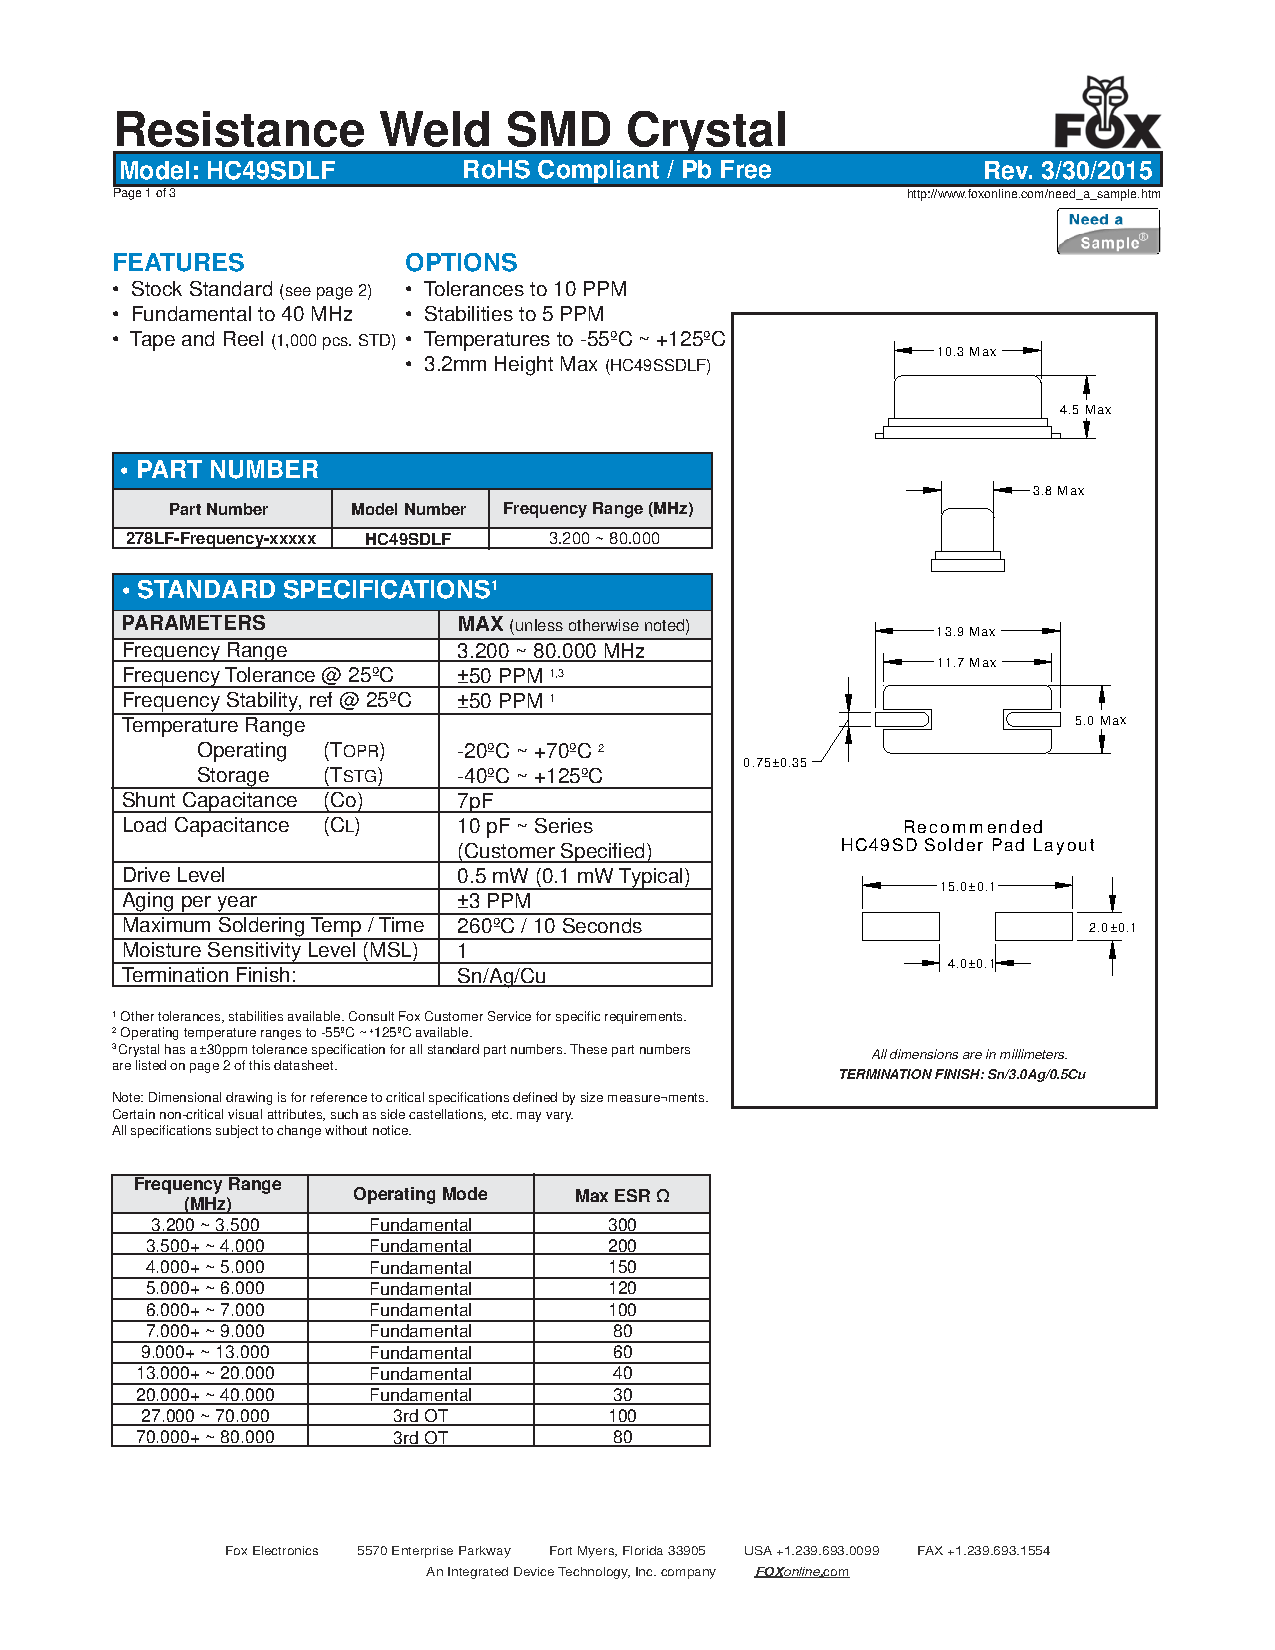
\includegraphics[page=1, width=.2\textwidth, clip, trim=15.25cm 18cm 2.75cm 8cm]{assets/datasheet/1911271.pdf}
	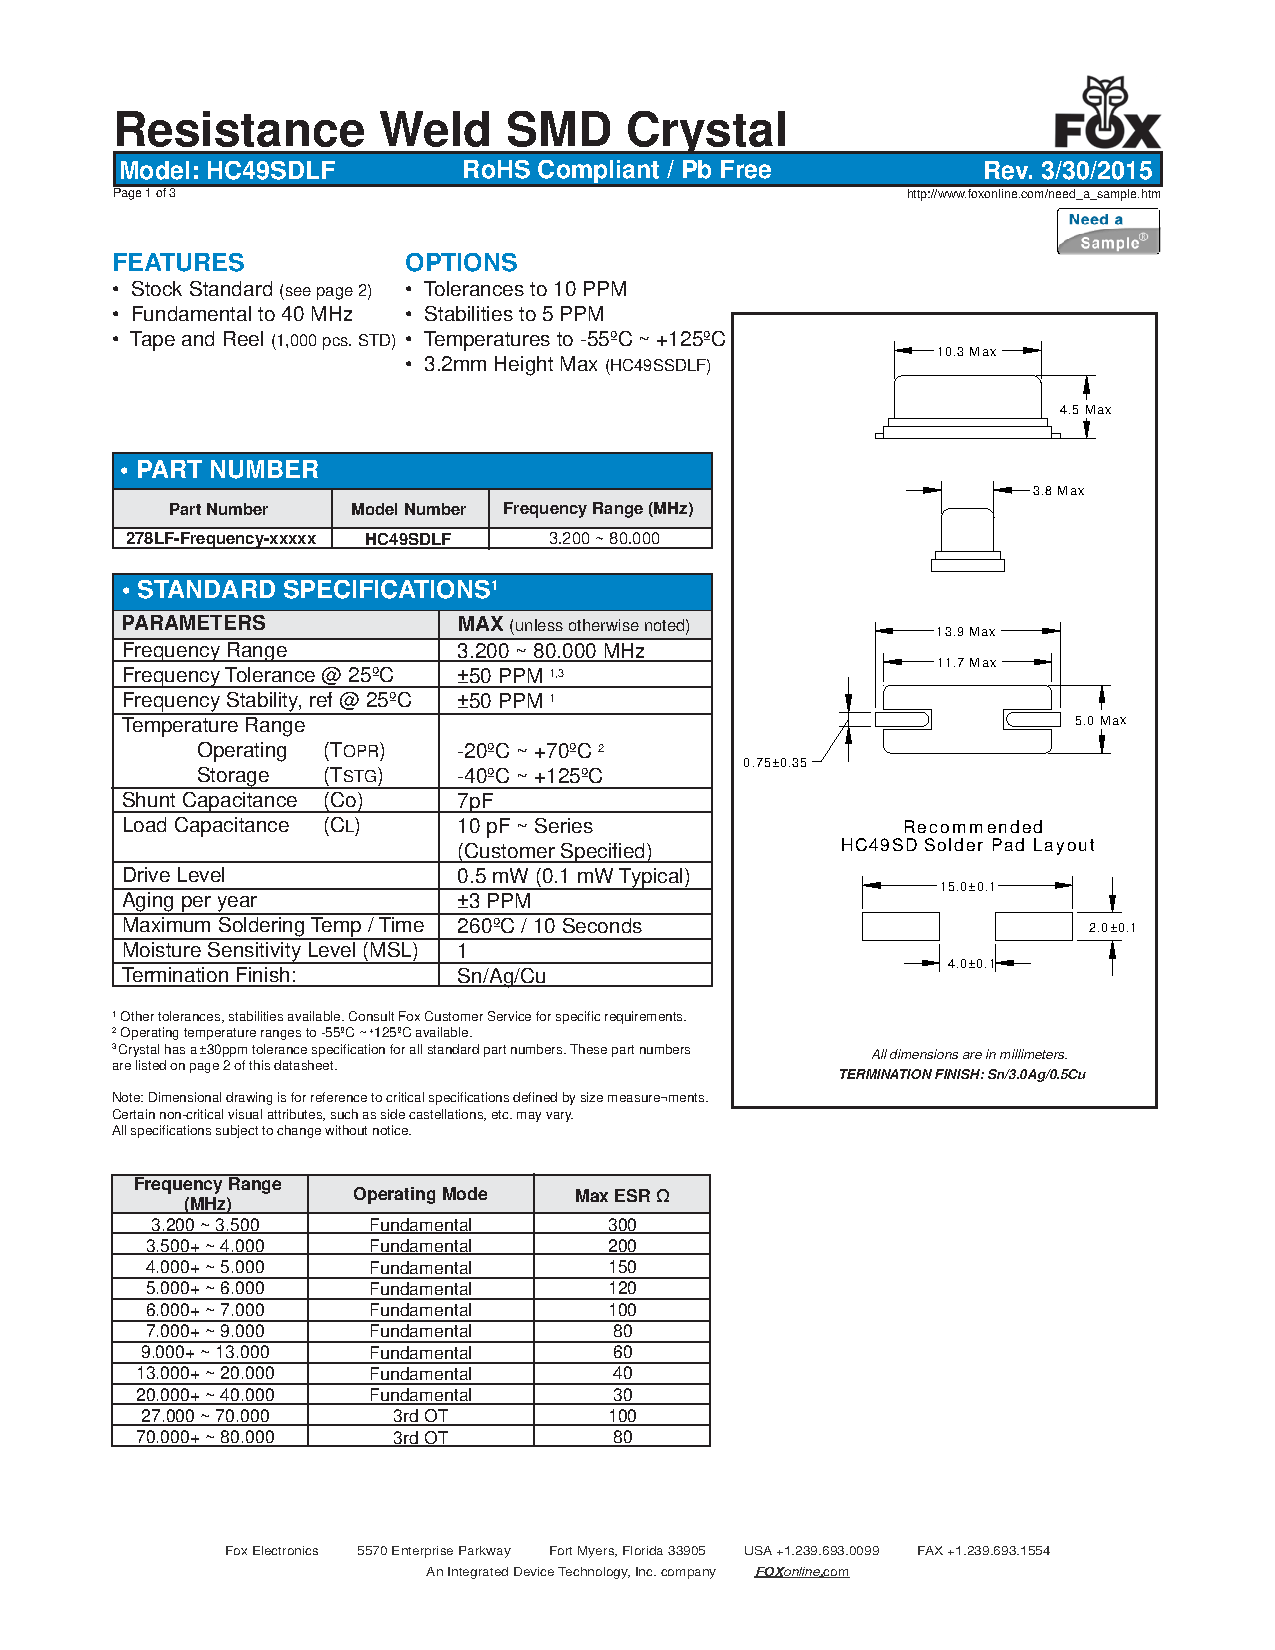
\includegraphics[page=1, width=.2\textwidth, clip, trim=14.75cm 20cm 2.75cm 5.5cm]{assets/datasheet/1911271.pdf}
	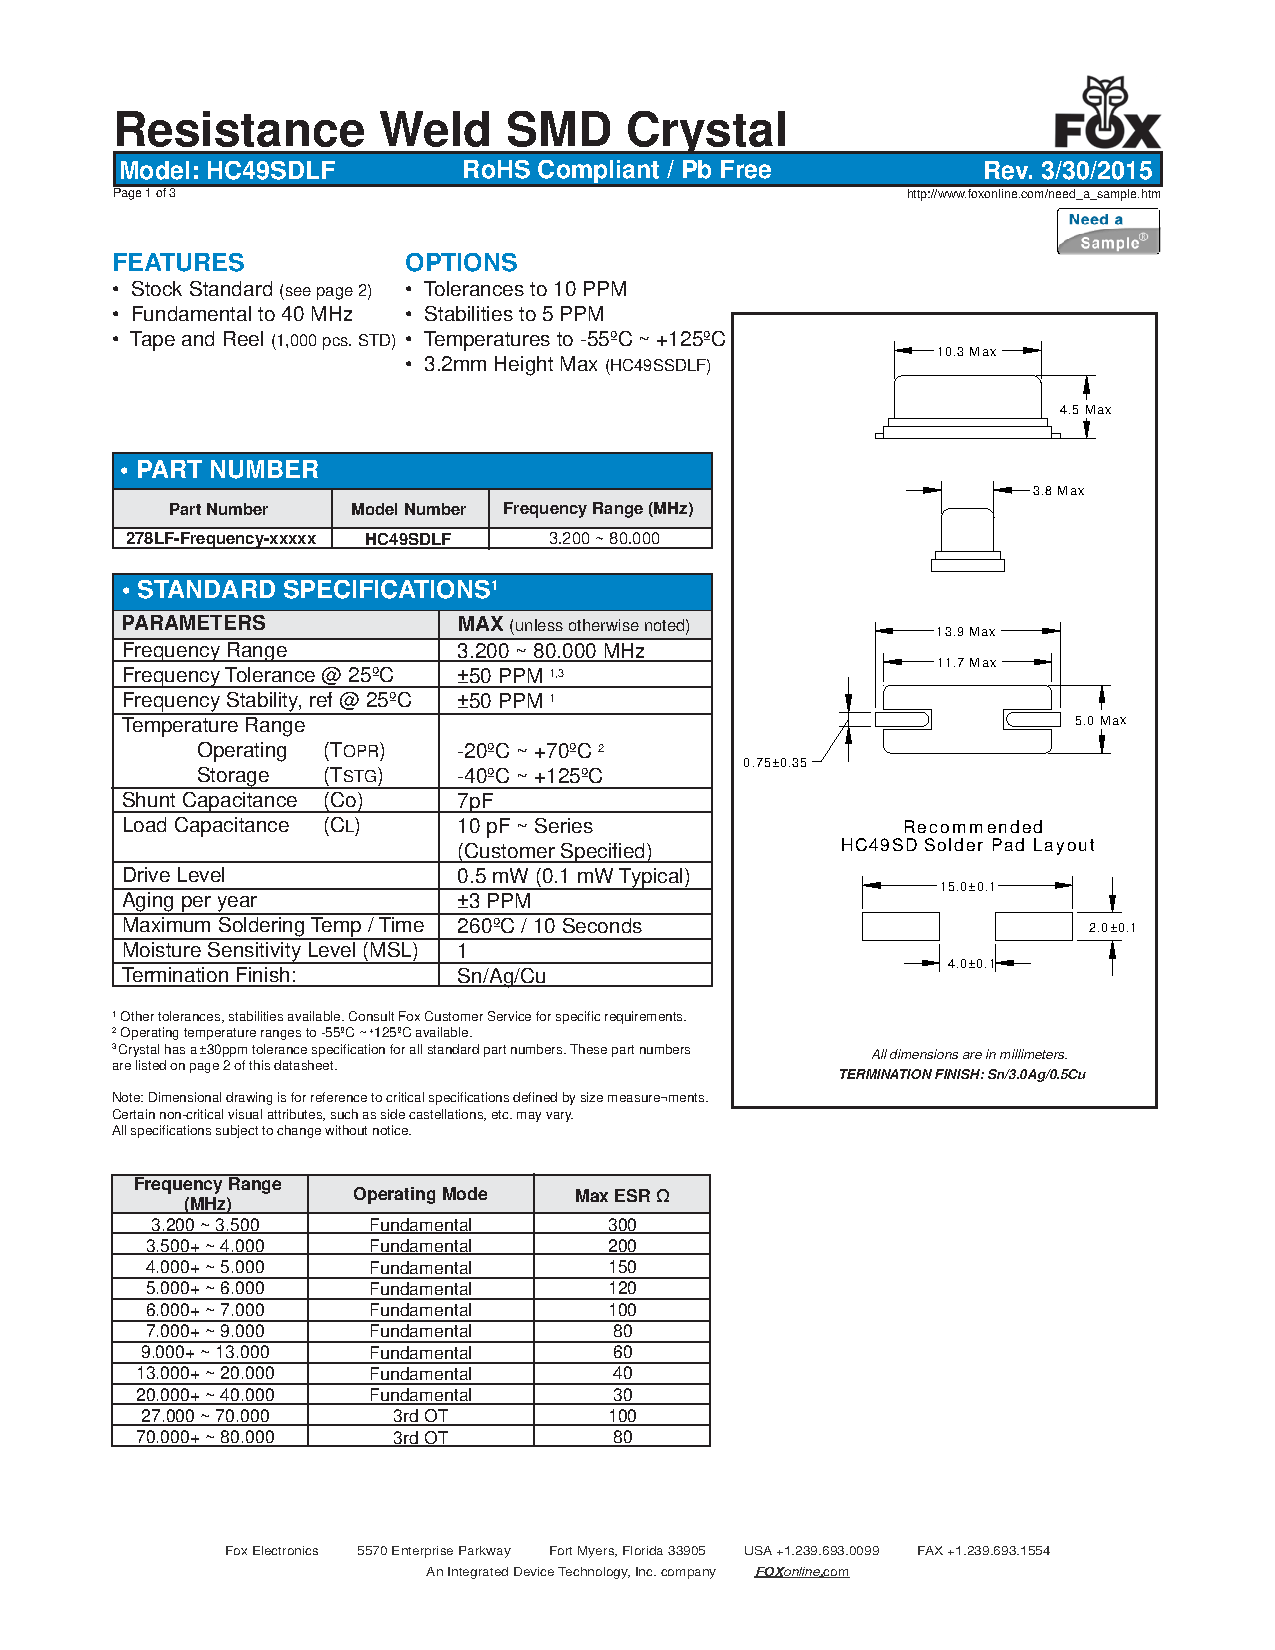
\includegraphics[page=1, width=.2\textwidth, clip, trim=14cm 11cm 2.25cm 13cm]{assets/datasheet/1911271.pdf}
	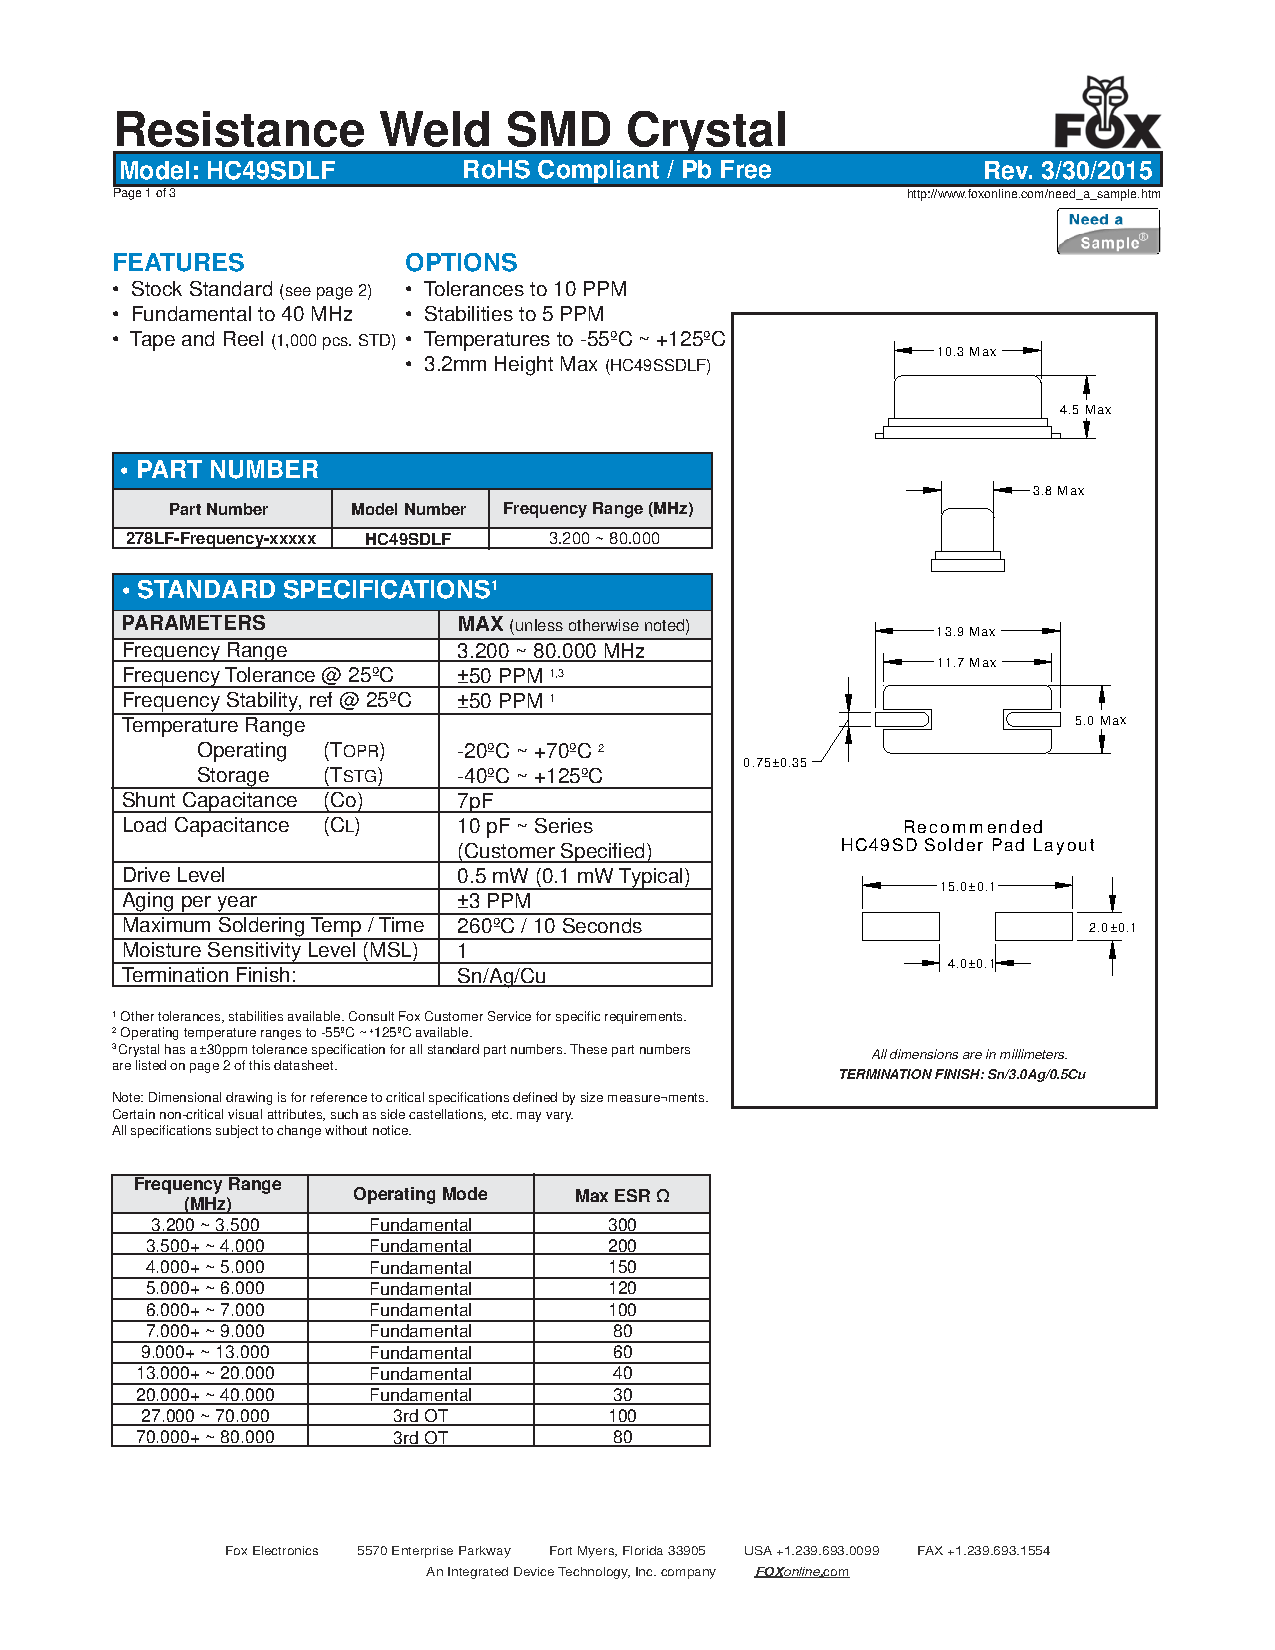
\includegraphics[page=1, width=.2\textwidth, clip, trim=12.5cm 14.5cm 2.5cm 10cm]{assets/datasheet/1911271.pdf} \\
	\caption[Caption for LOF]{
            \begin{inparaitem}[\phantom{\qquad}$\circ$]
                \item Allez à l'option $Tools \rightarrow New Blank Component$. \\
                \item Allez à l'option $Tools \rightarrow IPC Compliant Footprint Wizard...$. \\
                \item Depuis la boîte de dialogue $IPC Compliant Footprint Wizard$ ; allez à l'option $Next$, sélectionner l'élement $CHIP$ (Capacitor, Inductor, Resistor) ; allez à l'option $Next$, remplicer puis valider. \\
		\item Sauvegardez.
	    \end{inparaitem}
	}
\end{figure}

Pour le composant \href{http://www.farnell.com/datasheets/2325487.pdf\#page=3}{PTSA 1.5/2-3,5-Z} ci-suivant :

\begin{figure}[ht]
	\centering
	\includegraphics[page=3, width=.3\textwidth, clip, trim=13cm 20cm 3cm 5.75cm]{assets/datasheet/2325487.pdf}
	\includegraphics[page=3, width=.3\textwidth, clip, trim=7cm 13.5cm 7cm 12cm]{assets/datasheet/2325487.pdf} \\
	\caption[Caption for LOF]{
            \begin{inparaitem}[\phantom{\qquad}$\circ$]
                \item Allez à l'option $Tools \rightarrow New Blank Component$. \\
                \item Allez à l'option $Tools \rightarrow IPC Compliant Footprint Wizard...$. \\
		\item Sauvegardez.
	    \end{inparaitem}
	}
\end{figure}

\subsection{Board}
Allez à l'option $File \rightarrow New Pcb$. \\
Allez à l'option $Edit \rightarrow Origin \rightarrow Set$ et placer le point origine au bord inférieur gauche. \\
Allez à l'option $Tools \rightarrow Grid Manager$ ou pressez \Ctrl + \keystroke{G}. \\
Depuis la boîte de dialogue $Grid Manager$ ; allez à l'option $Menu$, sélectionner l'élement $Add Cartesian Grid$ puis valider. \\
Allez à l'option $View \rightarrow Board Planning Mode$. \\
Allez à l'option $Design \rightarrow Edit Board Shape$ afin de dimensionner la carte. \\
Allez à l'option $View \rightarrow 2D Layout Mode$. \\

% Polygon Pour - Bottom Layer

\end{document}
